\documentclass[sigplan,screen]{acmart}
\let\Bbbk\relax
\usepackage{amsmath, amsfonts, amssymb}
\usepackage{graphicx}
\usepackage{pmboxdraw}
\usepackage{hyperref}
\usepackage{listings}
\usepackage[acronym]{glossaries}
\makeglossaries
\usepackage{geometry}
\geometry{margin=1in}
\usepackage{tikz}
\usetikzlibrary{shapes.geometric, shapes.multipart, arrows.meta, positioning, calc}

\tikzstyle{startstop} = [rectangle, rounded corners, minimum width=3cm, minimum height=1cm,text centered, draw=black, fill=gray!20]
\tikzstyle{process} = [rectangle, minimum width=3cm, minimum height=1cm, text centered, draw=black, fill=blue!10]
\tikzstyle{decision} = [diamond, aspect=2, draw=black, fill=orange!20, text centered]
\tikzstyle{arrow} = [thick, ->, >=stealth]

% Manually define \xRightarrow since it's not working
\newcommand{\xRightarrow}[1]{\overset{#1}{\Rightarrow}}

% Manually define JSON listing format
\lstdefinelanguage{json}{
    basicstyle=\normalfont\ttfamily,
    numbers=left,
    numberstyle=\scriptsize,
    stepnumber=1,
    numbersep=8pt,
    showstringspaces=false,
    breaklines=true,
    frame=lines
}

\newglossaryentry{CAMS}{
  name={content-addressed module system},
  description={A module system where each module is uniquely identified by the cryptographic hash of its content and its declared dependencies. This guarantees immutability and supports decentralized resolution, verification, and reproducibility}
}

\newglossaryentry{MerkleTree}{
  name={Merkle tree},
  description={A cryptographic data structure where each non-leaf node is a hash of its children. Used for content verification and ancestry tracking in the module system.}
}

\newglossaryentry{Finalization}{
  name={finalization},
  description={The process of resolving all symbolic references in a module to their content-addressed identities, yielding a fully closed Merkle root.}
}

\newglossaryentry{SemanticVersioning}{
  name={Semantic Versioning (semver)},
  description={A versioning scheme using major, minor, and patch numbers (e.g., 1.2.3), often used for compatibility tracking in package managers.}
}

\newglossaryentry{DHT}{
  name={distributed hash table},
  description={A decentralized storage layer that maps content hashes or identifiers to locations or values across a peer-to-peer network.}
}

\newglossaryentry{Resolution}{
  name={resolution},
  description={The process of binding a symbolic identifier to its fully qualified content-addressed definition within the current ancestry context.}
}

\newglossaryentry{ContentAddressing}{
  name={content addressing},
  description={Identifying data by its hash rather than by name or location, allowing for immutable and verifiable references.}
}

\newglossaryentry{Shadowing}{
  name={shadowing},
  description={When a child module defines a symbol that overrides or hides a symbol from an ancestor module during inheritance.}
}

\newglossaryentry{AncestryGraph}{
    name={ancestry graph},
    description={A directed acyclic graph (DAG) representing the inheritance and dependency relationships between modules. Each node corresponds to a module, and each edge indicates an import or inheritance link. The ancestry graph is used during resolution to determine the order in which modules and symbols are composed or overridden.}
}

\newglossaryentry{Provenance}{
    name={provenance},
    description={The origin and historical lineage of a module or data artifact. In content-addressed systems, provenance includes the ancestry chain of dependencies, authorship, and the verifiable transformations that led to a module's current state. Provenance supports auditability, reproducibility, and trust in distributed systems}
}

\newglossaryentry{HashBomb}{
  name={hash bomb},
  description={A malicious module structure designed to overwhelm a resolution engine by creating an extremely large number of distinct but structurally similar hashes, often through slight content variations, leading to excessive memory or compute consumption during Merkle tree construction or verification}
}

\newglossaryentry{ExcessiveFanout}{
  name={excessive fan-out},
  description={A pathological module structure in which a single module imports an unusually large number of immediate dependencies, increasing the risk of performance degradation or denial-of-service during resolution}
}


\title{Merkle Tree-Based Inheritance for Decentralized Module Systems}

\author{S. C. Dunn}
\email{starlabsactual@gmail.com}
\date{\today}

\keywords{Merkle Trees, Module Inheritance, Content-Addressed Systems, Decentralized Systems}

\begin{CCSXML}
<ccsConcept>
    <conceptID>10010520</conceptID>
    <conceptDesc>Software and its engineering~Software architectures</conceptDesc>
</ccsConcept>
<ccsConcept>
    <conceptID>10010581</conceptID>
    <conceptDesc>Software and its engineering~Software dependability</conceptDesc>
</ccsConcept>
<ccsConcept>
    <conceptID>10010543</conceptID>
    <conceptDesc>Software and its engineering~Software version control</conceptDesc>
</ccsConcept>
<ccsConcept>
    <conceptID>10011007</conceptID>
    <conceptDesc>Computing methodologies~Cryptography</conceptDesc>
</ccsConcept>
<ccsConcept>
    <conceptID>10010525</conceptID>
    <conceptDesc>Software and its engineering~Software libraries</conceptDesc>
</ccsConcept>
<ccsConcept>
    <conceptID>10010663</conceptID>
    <conceptDesc>Software and its engineering~Programming languages</conceptDesc>
</ccsConcept>
<ccsConcept>
    <conceptID>10010661</conceptID>
    <conceptDesc>Software and its engineering~Software maintenance</conceptDesc>
</ccsConcept>
<ccsConcept>
    <conceptID>10011001</conceptID>
    <conceptDesc>Computing methodologies~Distributed computing</conceptDesc>
</ccsConcept>
<ccsConcept>
    <conceptID>10010504</conceptID>
    <conceptDesc>Software and its engineering~Modular programming</conceptDesc>
</ccsConcept>
<ccsConcept>
    <conceptID>10010528</conceptID>
    <conceptDesc>Software and its engineering~Software configuration management</conceptDesc>
</ccsConcept>
<ccsConcept>
    <conceptID>10010529</conceptID>
    <conceptDesc>Software and its engineering~Software package management</conceptDesc>
</ccsConcept>
\end{CCSXML}

\begin{document}

\begin{abstract}
In this paper, we introduce a novel approach to module inheritance and dependency resolution in distributed systems using Merkle trees. This method ensures deterministic finalization, secure content-based identification, and scalability in module registration and resolution. We discuss how Merkle tree-based inheritance addresses key challenges such as the diamond problem, ambiguity in dependency resolution, and the need for secure, decentralized module registries. Our method builds upon content-addressable hashing and authenticated data structures to ensure tamper-resistance and efficient verification of inheritance, suitable for peer-to-peer module execution platforms. We provide formal definitions, proofs, and runtime behaviors that demonstrate the practicality of this method in real-world decentralized systems. Our approach is implemented within the Tangl system, a distributed platform for managing decentralized modules, providing a foundation for flexible and secure module versioning.
\end{abstract}

\maketitle

\section{Introduction}

Module systems are fundamental to modern software development, enabling developers to create reusable components that can be seamlessly integrated into larger systems. In distributed environments, where modules can be authored, shared, and executed by diverse entities, managing dependencies and inheritance becomes increasingly complex. Traditional approaches to module inheritance often rely on fixed hierarchical structures or manual dependency resolution, leading to ambiguity and inefficiency \cite{cardelli1996}.

In decentralized systems, the necessity for a reliable, transparent, and scalable method to handle module dependencies is paramount. Centralized dependency resolution systems face limitations, including performance bottlenecks, trust issues, and challenges with versioning and compatibility \cite{decan2017}. Moreover, the absence of a single authority for managing dependencies heightens the risk of conflicts, version mismatches, and errors in module resolution. In the absence of clear guarantees, developers often resort to manual dependency resolution or depend on unreliable third-party services.

\glspl{MerkleTree} offer a robust solution to these challenges by providing a cryptographically secure method to verify content and resolve dependencies in a distributed setting. Merkle tree-based inheritance of modules using \gls{ContentAddressing} facilitates a scalable and verifiable approach to determining module relationships, allowing modules to inherit behavior and data from other modules in a secure and deterministic manner. This paper presents a Merkle tree-based inheritance model that addresses these issues, ensuring predictable, conflict-free inheritance resolution.

We define modules generically in this paper, though a specific realization of this model (including the Knot abstraction) is detailed in the Tangl project \cite{tangl}.

\section{Background}
\label{sec:background}

Managing module inheritance and dependencies in decentralized systems is a complex challenge. In such systems, modules are typically authored and maintained by independent parties, which complicates traditional mechanisms of dependency resolution. Unlike centralized systems where a single authority can enforce consistency, decentralized systems require a more flexible, verifiable, and autonomous method of resolving dependencies and managing module inheritance.

Traditional inheritance models, such as those used in object-oriented programming (OOP), assume a fixed, centralized hierarchy \cite{hewitt1977}. These models do not scale well in distributed environments, where the dependencies and inheritance structures are more fluid and subject to change. Furthermore, the centralized nature of traditional inheritance can create bottlenecks, as all module resolutions pass through a single point of failure. In contrast, decentralized systems require solutions that allow for module resolution and dependency tracking without relying on a central authority.

In content-addressed distributed systems, modules are identified by cryptographic hashes rather than names or locations, which makes traditional dependency resolution strategies impractical. The system must ensure that all parties have a consistent view of the module graph, even as modules evolve over time. Merkle trees provide an elegant solution for this challenge by enabling efficient and secure verification of the contents and relationships between modules \cite{merkle1987}. Merkle trees allow for modular and hierarchical verification: by hashing both the contents of a module and its relationship to other modules, Merkle trees ensure that the integrity of the system can be verified with minimal computational overhead.

Module inheritance in such a system refers to the process by which new modules can be derived from existing ones, with the ability to reuse, extend, or override functionality from parent modules. This inheritance is not managed through a fixed hierarchy but is instead encoded in the module's content hash, providing a decentralized, flexible, and verifiable method for composing new modules. By leveraging content addressing and Merkle trees, inheritance in this context is automatically traceable, immutable, and resistant to tampering.

The use of Merkle trees for inheritance also facilitates the implementation of \glspl{DHT} (DHTs) and other decentralized lookup methods, ensuring that module relationships and dependencies can be resolved efficiently without central coordination. This approach supports greater scalability, fault tolerance, and security in distributed systems, making it a promising solution for managing module inheritance in large-scale decentralized applications.

\section{Related Work and Motivation}
Several decentralized systems, such as IPFS, Git, and package managers like npm and Cargo, have addressed aspects of content-addressable storage and versioning \cite{benet2014}\cite{git}\cite{cargo_docs}\cite{npm_docs}. These systems use cryptographic hashes to ensure the integrity of module but do not provide a formalized mechanism for handling inheritance or dependencies. This paper builds upon these systems by introducing a Merkle tree-based inheritance model, where module dependencies and inheritance relationships are captured in a cryptographically secure and deterministic manner.

% hyphen in Ethereum to fix word wrap
Existing decentralized dependency systems like Ether-eum's smart contracts provide basic inheritance models, but they often suffer from issues such as the diamond problem, where multiple inheritance paths can create ambiguity \cite{solidity_inheritance}\cite{snyder1986}. Our approach resolves this by leveraging Merkle trees to explicitly define the resolution order for every inherited symbol, guaranteeing determinism and consistency across all executions.

\section{Challenges Addressed by Merkle Tree-Based Inheritance}
\label{sec:challenges}

The Merkle tree-based inheritance model employed in this system addresses several classical challenges associated with inheritance and module composition. The following subsections describe how this model resolves these issues through cryptographic hashes, content-\\addressable structures, and canonical ordering.

\subsection{The Diamond Problem}

A common challenge in multiple inheritance systems is the diamond problem, where a module inherits from two parents that themselves share a common ancestor \cite{snyder1986}. This can cause ambiguity in the application of inherited logic or data.

In the Merkle inheritance model, all parent modules are identified by their content hash. The ancestry tree is computed using a topological traversal, and duplicate content hashes are merged. Thus, a shared ancestor is represented once in the Merkle tree, eliminating redundant initialization or conflicting resolutions.

For example, consider the following inheritance structure:
\[
\text{Module } F \rightarrow \{D, E\}, \quad D \rightarrow \{A, B\}, \quad E \rightarrow \{A, C\}
\]
The module $A$ will appear only once in the computed Merkle tree of $F$, ensuring that all inherited elements from $A$ are unified without duplication or ambiguity.

\subsection{Ambiguity in Parent Resolution}

In traditional inheritance models, ambiguity can arise when multiple inheritance paths lead to similar or conflicting methods or fields, often requiring manual disambiguation \cite{python_mro}. In contrast, Merkle tree-based inheritance defines a \textbf{canonical order} for ancestry resolution that eliminates ambiguity through a deterministic, verifiable process. The order is determined by the following principles:

\begin{itemize}
    \item \textbf{Lexicographic ordering of content hashes}: The content hashes of modules are used to establish a consistent order, ensuring that modules with the same ancestry are resolved based on the lexicographical comparison of their hashes.
    \item \textbf{Topological sorting of the directed acyclic graph (DAG)}: The directed acyclic graph formed by module imports is topologically sorted to respect the dependency relationships between modules. This guarantees that a module’s ancestors are processed in a consistent, hierarchical order.
    \item \textbf{Optional rule-based tie-breaking}: In cases where modules are equally prioritized in the lexicographic or topological order, tie-breaking can be applied using rules such as depth-first priority or timestamp-based preference. These rules provide additional determinism and help resolve any conflicts when multiple paths lead to the same module.
\end{itemize}

This canonical order ensures that each module’s ancestry is resolved in a unique and consistent manner, promoting both predictability and verifiability in the resolution process.

\subsection{Cyclic Dependencies}
\label{sec:cyclic-deps}

The use of content addressing and Merkle trees inherently prevents cyclic inheritance, ensuring a well-\\structured and acyclic dependency graph \cite{benet2014}. Since each module's identity is determined by the content hashes of its declared imports, the formation of a cycle would create a circular hash dependency. This is mathematically impossible due to the properties of cryptographic hash functions such as SHA-256, which are one-way functions and inherently acyclic. As a result, any attempt to form a cycle in the module graph would result in an invalid state, ensuring that dependencies remain acyclic and verifiable.

\subsection{Tamper Resistance and Integrity}

Each finalized module inherits not only behavior but also a cryptographically verifiable proof of ancestry. Because the Merkle tree includes all transitive ancestors in a tamper-proof structure, any modification to an ancestor will:

\begin{itemize}
    \item Alter the content hash.
    \item Invalidate the Merkle root.
    \item Propagate changes upward, altering all dependent modules.
\end{itemize}

This ensures referential transparency and immutability across distributed environments.

\subsection{Efficient Validation and Caching}

Once a module is finalized, its computed Merkle tree and hash can be persisted. This enables downstream modules to:

\begin{itemize}
    \item Reuse validated ancestry trees without recomputation.
    \item Quickly verify conformance and inheritance during finalization or execution.
    \item Improve scalability in distributed systems by caching shared subtrees.
\end{itemize}

The use of content-addressable structures ensures that identical inheritance trees yield identical hashes, supporting efficient distributed caching and deduplication.

\section{Comparison with Existing Systems}
\label{sec:comparison}

The module resolution model described in this paper, built on symbolic references, lexical \gls{Shadowing}, and content-addressed identifiers, marks a substantial departure from existing approaches to software composition. Traditional systems such as \texttt{npm}, \texttt{Cargo}, and \texttt{pip} resolve dependencies through a centralized registry and a version constraint solver, while reproducibility-focused systems like Nix and IPFS use content hashes and store-path resolution. By contrast, our model introduces a novel runtime-based resolution strategy based on deterministic symbol lookup over a hierarchical, immutable reference graph.

These differences are reflected in our prototype implementation, \textit{Tangl}, which operationalizes the model in a distributed setting. In Tangl, modules reference other modules via symbolic names bound to content hashes in a reference map. The resolution of a symbol is deferred until a dedicated resolve phase during runtime, during which all transitive bindings are located, either from local cache or the network. This deferred resolution strategy enables lazy loading, caching optimizations, and precise control over symbol scope.

Unlike version-based systems, which use constraint solvers to select from a range of candidate versions, our model treats resolution as a lexical and symbolic process. The order and specificity of imports determine which symbol is selected. For example, a module that imports \texttt{b} followed by \texttt{a}, then calls \texttt{foo()}, will resolve the call to \texttt{b.foo}, unless \texttt{a.foo} was explicitly imported using a more granular import like \texttt{import(a.foo)}, in which case \texttt{a.foo} takes precedence. This mechanism eliminates ambiguity and avoids the need for version negotiation or lockfiles, while still supporting fine-grained override and shadowing semantics.

The resolve phase, as implemented in Tangl’s runtime, recursively traverses the reference map to locate all required content-hashed modules. This traversal is deterministic and requires no external coordination, ensuring reproducibility and verifiability. Once all required modules are located, execution can proceed with a complete and locally available resolution environment. This allows Tangl to function efficiently in distributed and offline contexts without sacrificing correctness or transparency.

By treating linking and resolution as symbolic substitution within a content-addressed graph, the model eliminates many of the ambiguities and global coordination problems that arise in versioned dependency systems. The Tangl prototype demonstrates how this model can be implemented in practice, offering a viable path forward for verifiable, distributed software composition.

\section{Merkle Tree-Based Inheritance Model}
\subsection{Merkle Trees}
A Merkle tree, or hash tree, is a binary tree in which each leaf node represents a hash of a data block, and each non-leaf node represents a hash of its children. This structure allows for efficient and secure verification of the integrity of large data structures. In the context of module inheritance, Merkle trees can be used to represent the relationships between modules and their dependencies.

\subsection{Content-Addressed Module Systems}
\label{sec:content-addressed-module-systems}

We define a \gls{CAMS} as a module system in which each module is uniquely identified by a cryptographic hash of its content and its declared dependencies. Unlike traditional systems that rely on names, versions, or centralized registries, content-addressed systems derive identity directly from the structure and substance of the module.

This approach enables several key properties essential to decentralized environments:
\begin{itemize}
    \item \textbf{Immutability:} Modules cannot be altered without changing their identity.
    \item \textbf{Tamper Resistance:} Integrity can be verified independently by re-computing hashes.
    \item \textbf{Reproducibility:} Module graphs are guaranteed to resolve the same way on any machine.
    \item \textbf{Decentralized Resolution:} Modules can be retrieved and validated without reliance on a central authority.
\end{itemize}

In this paper, we use the term \textit{content-addressed module system} to refer to any system that satisfies these properties and supports deterministic, verifiable module inheritance.

\subsection{Module Representation}
In our model, each module is represented as a leaf node in the Merkle tree structure. The module's content, including its code, metadata, and declared dependencies, is cryptographically hashed to generate a unique identifier, known as the \textit{module ID}. This identifier is derived from the module’s content-addressed structure, meaning that any modification to the module, whether it's a change in code, metadata, or dependencies, will result in a different hash and, consequently, a different module ID.

This content-addressed approach guarantees the integrity of the module, as any change in its content will be reflected in the hash. Additionally, it provides traceability, as the history of changes to the module can be traced back through its hash history in the Merkle tree. The Merkle tree structure ensures that these changes are efficiently verifiable and can be resolved deterministically across distributed systems.

\subsection{Inheritance Mechanism}
Inheritance in our model is represented by linking modules through their Merkle tree hashes. A module can inherit from another by referencing the parent module's content-addressed ID. This reference establishes a clear and verifiable relationship between modules, ensuring that all dependencies are properly accounted for and that the inheritance hierarchy remains consistent. The use of Merkle hashes ensures that any change in the parent module’s content is reflected in the child module’s identity, providing strong guarantees of integrity and traceability across the entire inheritance tree.

\subsection{Canonicalization of Inheritance Trees}
\label{sec:canonicalization}

Let each module import zero or more parent modules via symbolic import paths. We define an \textit{ancestry DAG} $\mathcal{G}_M = (V, E)$, where $V$ are module content hashes and $E$ are edges representing declared imports.

To compute a canonical inheritance sequence:

\begin{enumerate}
  \item Construct $\mathcal{G}_M$ transitively from all imports.
  \item Topologically sort $\mathcal{G}_M$, using content hash order as a deterministic tie-breaker.
  \item Traverse the resulting DAG and apply a fixed-point de-duplication.
\end{enumerate}

Formally, we define the linearized ancestry list $\mathcal{L}_M$ of a module $M$ as:

\[
\mathcal{L}_M = \text{fix}(\lambda L. \text{dedup}(\bigcup_{\text{parent} \in M.\text{imports}} \mathcal{L}_{\text{parent}} \cup \{M\}))
\]

This process produces a content-addressed, deterministically ordered, duplicate-free ancestry list. Cyclic imports are prevented by the deterministic and immutable nature of the \gls{Finalization} process.

\subsection{Clarification of Inheritance Semantics and Edge Cases}

While the formal model for inheritance in Merkle tree-based systems provides a sound theoretical foundation, it is crucial to address practical scenarios, especially edge cases like circular dependencies or conflicting module versions. 

\subsubsection{Circular Dependencies}
\label{sec:circular-deps}

In our model, circular dependencies are inherently prevented by the resolution process. Since the system relies on content-addressed resolution and Merkle tree-based linking, each module must resolve all its symbols before finalization. If a cycle were to occur, one of the modules in the cycle would fail to resolve its symbols, as it would depend on the unresolved module, preventing the cycle from completing. 

This ensures that the module resolution process remains acyclic and predictable, with each module being independently resolvable before it is finalized and added to the module graph. Any attempt to resolve a cycle would trigger an error or warning to the developer, who would need to break the circular dependency manually, ensuring that the graph remains valid.

\subsubsection{Conflicting Module Versions}
\label{sec:conflicting-versions}

Conflicts arise when different modules depend on different versions of the same dependency. In traditional systems, this often results in version resolution errors or unexpected runtime behavior due to global state or shared environments. In contrast, our content-addressed inheritance model safely supports multiple versions of the same module coexisting within the same dependency graph.

Because each module is identified by a cryptographic content addressing hash, different versions naturally produce distinct, immutable identifiers. This ensures that even if multiple modules reference different versions of the same dependency, their imports remain isolated and unambiguous. The system does not attempt to merge these dependencies unless explicitly directed to do so by the developer.

When modules are executed in sandboxed runtimes, such as WebAssembly instances, this isolation extends to the runtime level, preventing symbol collisions and ensuring that internal state and behavior do not interfere across versions. Tools can further aid developers by exposing precise version paths during resolution, enabling awareness of transitive dependency trees and allowing version pinning or override declarations.

For example, two versions of the same module can be imported under separate names:
\begin{quote}
\texttt{import "crypto@1.2.0" as crypto\_v1;}\\
\texttt{import "crypto@2.0.1" as crypto\_v2;}
\end{quote}

By embracing this explicit, hash-based strategy, our system provides strong guarantees of reproducibility and safety, even in the presence of complex or divergent dependency graphs. Developers retain full control over which versions are used where, and tooling can report potential conflicts, overrides, or redundancies for better maintainability.

This approach makes version conflicts not a source of ambiguity, but an intentional, traceable design choice, supporting both fine-grained control and large-scale modular reuse.

\tikzset{
  module/.style={rectangle, draw=blue!50, fill=blue!10, thick, minimum width=2cm, minimum height=1.2cm},
  symbol/.style={rectangle, draw=black!80, fill=gray!10, thin, minimum width=1.6cm, minimum height=0.8cm},
  arrow/.style={-Stealth, thick},
  override/.style={dashed, thick, red!70}
}

\begin{figure}[ht]
\centering
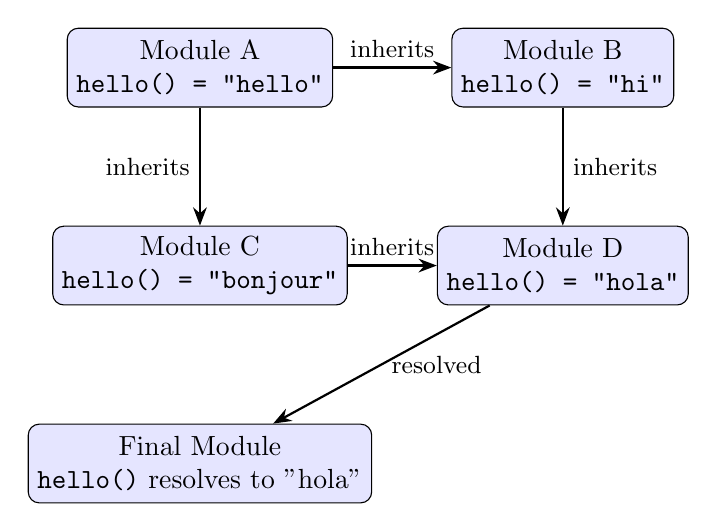
\begin{tikzpicture}[
  module/.style={draw, rounded corners, minimum width=2.5cm, minimum height=1cm, fill=blue!10, align=center},
  override/.style={->, thick, >=Stealth, color=black},
  node distance=1.5cm
]

% Nodes with align=center so \\ works
\node[module] (A) {Module A\\\texttt{hello() = "hello"}};
\node[module, right=of A] (B) {Module B\\\texttt{hello() = "hi"}};
\node[module, below=of A] (C) {Module C\\\texttt{hello() = "bonjour"}};
\node[module, below=of B] (D) {Module D\\\texttt{hello() = "hola"}};
\node[module, below=of C] (Final) {Final Module\\\texttt{hello()} resolves to "hola"};

% Arrows
\draw[override] (A) -- (B) node[midway, above] {\small inherits};
\draw[override] (A) -- (C) node[midway, left] {\small inherits};
\draw[override] (B) -- (D) node[midway, right] {\small inherits};
\draw[override] (C) -- (D) node[midway, above] {\small inherits};
\draw[override] (D) -- (Final) node[midway, right] {\small resolved};

\end{tikzpicture}
\caption{Merkle-based inheritance with multiple overrides. Module A defines \texttt{hello()}, which is overridden in B and C. D inherits from both B and C, and the final module resolves \texttt{hello()} from D.}
\label{fig:merkle-inheritance-example}
\end{figure}

\subsection{Formal Module Semantics}
\label{sec:formal-semantics}

The semantics of Merkle tree-based inheritance draw on foundational work in the semantics of module systems~\cite{dreyer2005module}, adapting traditional constructs such as imports, exports, and substitution to a decentralized, content-addressed setting. Each module is treated as a unit of encapsulation and composition, with Merkle roots representing immutable snapshots of the module’s symbol table and inheritance relationships forming a directed acyclic graph (DAG).

To reason about soundness and determinism, we model symbol resolution as a total function over a Merkle DAG, where shadowing and override precedence follow a deterministic merge strategy akin to linear extension of the ancestry graph. This is similar in spirit to mixin module semantics~\cite{ancona2003foundations}, where module composition preserves override order and type safety. Our system ensures that for any well-formed module graph, symbol resolution is unambiguous and stable under extension, key properties necessary for compositionality.

We define a symbolic resolution trace as a path from the querying module through its ancestry DAG to the module that defines a symbol. This trace is unique (due to deterministic merge rules) and reproducible (due to hash-based identity), enabling both static reasoning and runtime validation.

Future work will extend this semantic model into a formal calculus for decentralized modules, allowing proofs of compositional soundness, override determinism, and evaluation invariance over distributed execution contexts.

\subsection{Real-World Use Cases and Interoperability}
\label{sec:use-cases}

To illustrate the practicality of Merkle tree-based inheritance, we present a series of real-world development scenarios that highlight the system’s resolution semantics, support for interoperability, and improvements over existing dependency systems.

\paragraph{Use Case 1: Overriding and Forking a Dependency}

Suppose a developer uses a module \texttt{libA} that defines a function \texttt{validate()}. In a traditional ecosystem like npm or Cargo, modifying \texttt{validate()} requires forking the entire package and updating downstream dependencies manually. In contrast, our system allows a new module \texttt{libB} to inherit from \texttt{libA} and override only the \texttt{validate()} function. All unchanged behavior remains inherited by hash, and tools can trace the exact override \gls{Provenance} via ancestry inspection. This reduces friction when applying custom patches without sacrificing reproducibility.

\paragraph{Use Case 2: Semantic Version Resolution and Module Inflation}

Semantic versioning in npm allows flexible version specifiers (e.g., \verb#^1.2.3#), often resulting in projects resolving to multiple versions of the same package. This can bloat dependency trees and cause non-deterministic behavior~\cite{pinckney2023largescale}. In our system, \gls{SemanticVersioning} references are resolved to content hashes before finalization, ensuring that the final build is content-addressed and deterministic. Each version resolution is recorded explicitly, enabling debugging and reproducibility, even when upstream modules evolve.

\paragraph{Use Case 3: Integration with npm, Cargo, and pip}

To bridge existing ecosystems, we define import adapters for package managers such as npm, Cargo, and pip. These adapters translate semver-based imports into finalized Merkle roots at the time of module finalization (See Figure~\ref{fig:translation-workflow}). For instance:

\begin{lstlisting}[language=json,caption={npm-style import resolved to content hash},label={lst:npm-to-merkle}]
"dependencies": {
  "left-pad": "^1.3.0"
}
\end{lstlisting}

is resolved via a Merkle-aware registry to:

\begin{lstlisting}[language=json]
"dependencies": {
  "left-pad": "merkle:9a3f...12e7"
}
\end{lstlisting}

Unlike traditional systems, this transformation is not stored in a lockfile. Instead, the finalized Merkle root of the module captures the complete and immutable dependency graph. This ensures reproducibility without introducing auxiliary metadata files and maintains full compatibility with deterministic builds and ancestry tracing.

\paragraph{Protocol for Handling Version Mismatches}

Content addressing enables multiple versions of the same module to coexist safely in the same dependency graph, as each version is identified by a unique hash. This removes the traditional constraint of globally singular versions and allows different ancestors to reference distinct versions without collision. When necessary, developers may intentionally override transitive dependencies by introducing an explicit wrapper module that inherits from the conflicting versions and reconciles any behavioral or interface discrepancies. These override semantics make conflict resolution composable and transparent, allowing developers to control shadowing behavior, expose specific symbols, or patch inconsistencies at defined boundaries. This approach eliminates ambiguity, avoids silent breakage, and supports reproducible and observable dependency graphs.

\begin{figure*}[t]
\centering
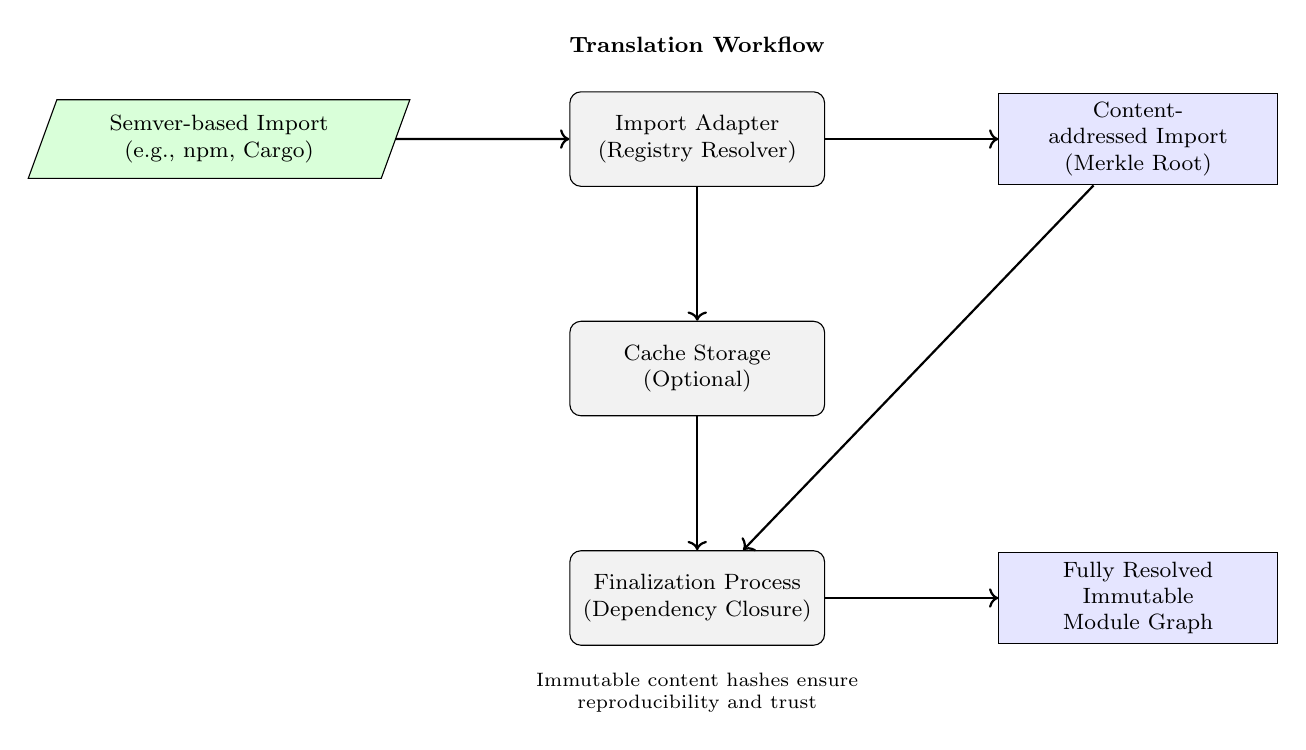
\begin{tikzpicture}[
  node distance=1.7cm and 2.2cm,
  every node/.style={font=\footnotesize},
  process/.style={rectangle, draw=black, fill=gray!10, rounded corners, minimum height=1.2cm, align=center, text width=3cm},
  data/.style={rectangle, draw=black, fill=blue!10, minimum height=1cm, align=center, text width=3.3cm},
  io/.style={trapezium, trapezium left angle=70, trapezium right angle=110, draw=black, fill=green!15, minimum height=1cm, align=center, text width=3.2cm},
  arrow/.style={->, thick}
]

% Nodes
\node[io] (source) {Semver-based Import\\ (e.g., npm, Cargo)};
\node[process, right=of source] (adapter) {Import Adapter\\ (Registry Resolver)};
\node[data, right=of adapter] (resolved) {Content-addressed Import\\ (Merkle Root)};
\node[process, below=of adapter] (cache) {Cache Storage\\ (Optional)};
\node[process, below=of cache] (finalize) {Finalization Process\\ (Dependency Closure)};
\node[data, right=of finalize] (output) {Fully Resolved\\ Immutable Module Graph};

% Arrows
\draw[arrow] (source) -- (adapter);
\draw[arrow] (adapter) -- (resolved);
\draw[arrow] (adapter) -- (cache);
\draw[arrow] (cache) -- (finalize);
\draw[arrow] (resolved) -- (finalize);
\draw[arrow] (finalize) -- (output);

% Labels
\node[above of=adapter, node distance=1.2cm] {\textbf{Translation Workflow}};
\node[below of=finalize, node distance=1.2cm, font=\scriptsize, align=center] {Immutable content hashes ensure\\ reproducibility and trust};

\end{tikzpicture}
\caption{Workflow for translating semver-based imports into Merkle-rooted content-addressed modules.}
\label{fig:translation-workflow}
\end{figure*}

\section{Formalization of Finalization}
\label{formalization-finalization}

Finalization refers to the process of resolving a module's dependencies and determining its final state. In our model, finalization is deterministic and injective, meaning that for a given set of inputs, there is a unique final state.

\subsection{Determinism}
Determinism ensures that the final state of a module is predictable and consistent. Given the same inputs, the finalization process will always produce the same result. This property is crucial for debugging and maintaining distributed systems.

\subsection{Injectivity}
Injectivity guarantees that each unique set of inputs results in a unique final state. This property prevents conflicts and ambiguities in module resolution, ensuring that modules are correctly and uniquely identified.

\subsection{Modules as Values}
\label{sec:modules-as-values}

In our model, a finalized module is treated as a first-class value with a well-defined structure. Each module is represented as a tuple:
\[
M = (C, T, A, P)
\]
where:

\begin{itemize}
    \item $C$ denotes the module’s content, which may be source code, bytecode, or any other serializable data.
    \item $T$ is a UNIX timestamp that records the moment of finalization (i.e. publication).
    \item $A$ is the author’s identifier, typically represented as a public key or cryptographic identity.
    \item $P = \{M_1, M_2, \ldots, M_n\}$ is the set of parent modules from which $M$ inherits. All parents must themselves be finalized prior to inclusion.
\end{itemize}

This tuple encapsulates both the internal semantics and external context of a module. The structure enables consistent hashing, resolution, and identity derivation across distributed systems. Throughout our semantics, we assume the presence of a cryptographic hash function $H(\cdot)$, for example, SHA-256, to ensure content-addressable integrity.

\subsection{Module Identity and Content Hashing}
\label{sec:module-identity}

The identity of a module is determined by both its internal content and its external context. To begin, we define a \textbf{content hash} that captures the internal semantics of the module independently of its ancestry:
\[
h_C = H(C)
\]
where $C$ represents the module's source content (including declarations, definitions, and symbol exports), and $H$ is a cryptographic hash function such as SHA-256. This ensures that any module with identical internal structure will produce the same $h_C$, regardless of its author or inherited dependencies.

To establish the final, globally unique identity of the module, we incorporate the content hash alongside its full provenance:
\[
h_M = H(h_C \, || \, T \, || \, A \, || \, H_{\text{merkle}}(P))
\]
Here, $T$ is a timestamp or logical clock, $A$ is the author's identifier (such as a public key or registry signature), and $H_{\text{merkle}}(P)$ is the Merkle root of the module’s transitive ancestry graph.

Together, these components ensure that changes to a module’s source code, ancestry, or metadata produce a distinct identity. This structure guarantees reproducibility, supports immutable caching, and underpins decentralized inheritance and resolution in content-addressed module systems.

\subsection{Ancestry and Merkle Root}

The ancestry of a module is defined as the transitive closure over its parent set:
\[
A(M) = \bigcup_{m \in P} \{m\} \cup A(m)
\]

To compute the ancestry root (See Figure~\ref{fig:merkle-ancestors}):
\begin{enumerate}
    \item Collect the final IDs $h_{m_i}$ of all ancestors in $A(M)$.
    \item Sort them lexicographically.
    \item Construct a balanced binary Merkle tree from this sorted list.
    \item Let $H_{\text{merkle}}(P)$ be the root hash of the resulting tree.
\end{enumerate}

This ordering guarantees deterministic ancestry representation and allows compact proofs of inclusion.

\subsection{Symbol Resolution}

Each module $M$ exports a set of named symbols:
\[
S_M = \{ s_i = (\text{name}, \text{value}, \text{type}) \}
\]

During finalization, $M$ computes a static resolution table:
\[
R_M : \text{name} \rightarrow \langle M_i, s_j \rangle
\]

For each symbol name, the table identifies the ancestor $M_i \in A(M)$ and the symbol $s_j$ it resolves to. Resolution is based on the canonical Merkle ordering of ancestors and is computed once, at finalization time.

\begin{figure*}[t]
\centering
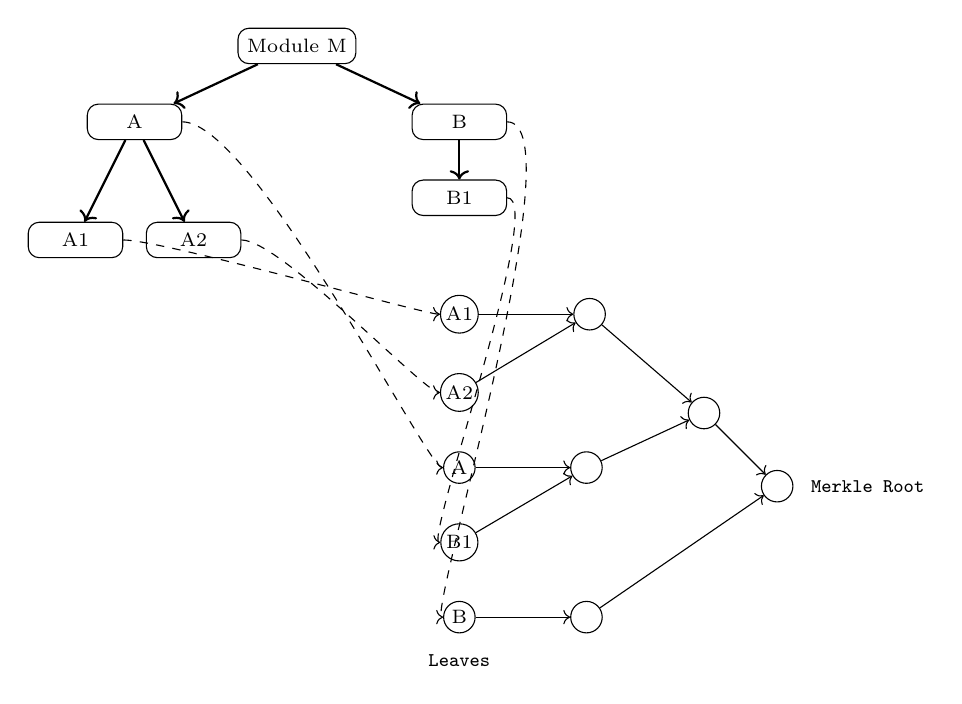
\begin{tikzpicture}[
  font=\scriptsize,
  box/.style={draw, rounded corners, minimum width=1.2cm, minimum height=0.45cm, align=center},
  hash/.style={draw, circle, minimum size=0.4cm, inner sep=1pt},
  node distance=0.5cm and 0.6cm,
  every node/.style={transform shape}
]

% Module inheritance tree (left)
\node[box] (m) {Module M};
\node[box, below left=0.5cm and 0.7cm of m] (a) {A}
[grow=down]
child {node[box] (a1) {A1}}
child {node[box] (a2) {A2}};

\node[box, below right=0.5cm and 0.7cm of m] (b) {B};
\node[box, below=of b] (b1) {B1};

\draw[->, thick] (m) -- (a);
\draw[->, thick] (m) -- (b);
\draw[->, thick] (a) -- (a1);
\draw[->, thick] (a) -- (a2);
\draw[->, thick] (b) -- (b1);

% Merkle tree (right side, compact)
\node[hash, below=1cm of b1] (l1) {A1};
\node[hash, below=of l1] (l2) {A2};
\node[hash, below=of l2] (l3) {A};
\node[hash, below=of l3] (l4) {B1};
\node[hash, below=of l4] (l5) {B};

% Internal nodes
\node[hash, right=1.2cm of l1] (h1) {};
\draw[->] (l1) -- (h1);
\draw[->] (l2) -- (h1);

\node[hash, right=1.2cm of l3] (h2) {};
\draw[->] (l3) -- (h2);
\draw[->] (l4) -- (h2);

\node[hash, right=1.2cm of l5] (h3) {};
\draw[->] (l5) -- (h3);

\node[hash, above right=0.4cm and 1.2cm of h2] (h4) {};
\draw[->] (h1) -- (h4);
\draw[->] (h2) -- (h4);

\node[hash, below right=0.9cm of h4] (root) {};
\draw[->] (h3) -- (root);
\draw[->] (h4) -- (root);

% Dashed lines mapping inheritance -> leaves
\draw[dashed, ->] (a1.east) .. controls +(right:0.5cm) and +(left:0.2cm) .. (l1.west);
\draw[dashed, ->] (a2.east) .. controls +(right:0.5cm) and +(left:0.2cm) .. (l2.west);
\draw[dashed, ->] (a.east)  .. controls +(right:0.9cm) and +(left:0.2cm) .. (l3.west);
\draw[dashed, ->] (b1.east) .. controls +(right:0.5cm) and +(left:0.2cm) .. (l4.west);
\draw[dashed, ->] (b.east)  .. controls +(right:0.9cm) and +(left:0.2cm) .. (l5.west);

% Labels
\node[right=0.1cm of root] {\texttt{Merkle Root}};
\node[below=0.15cm of l5] {\texttt{Leaves}};

\end{tikzpicture}
\caption{Mapping of transitive ancestors to Merkle leaf nodes and internal hash structure.}
\label{fig:merkle-ancestors}
\end{figure*}

\subsection{Named References and Registry Resolution}

Before finalization, parent references may be symbolic, e.g.:
\begin{verbatim}
import math/utils@1.2.0
\end{verbatim}

These are resolved by a registry function:
\[
\mathcal{R}: (\text{name}, \text{semver}) \rightarrow h_{M'}
\]

Once resolved, symbolic references are replaced by concrete module hashes and included in $P$, preserving all cryptographic guarantees.

\subsection{Finalization Algorithm}

Finalization is a total function:
\[
\mathcal{F}(C, T, A, \{r_1, \ldots, r_n\}) = h_M
\]

Where each $r_i$ is either:
\begin{itemize}
    \item a finalized module ID $h_{M_i}$, or
    \item a symbolic reference to be resolved through $\mathcal{R}$.
\end{itemize}

Finalization proceeds as:

\begin{enumerate}
    \item Resolve all symbolic references via $\mathcal{R}$.
    \item Ensure all $h_{M_i}$ are finalized and valid.
    \item Compute $A(M)$ and derive the sorted list of ancestor IDs.
    \item Compute $H_{\text{merkle}}(P)$ as the Merkle root over that list.
    \item Hash the module content: $h_C = H(C)$.
    \item Compute the final module ID:
    \[
    h_M = H(h_C \, || \, T \, || \, A \, || \, H_{\text{merkle}}(P))
    \]
\end{enumerate}

This procedure is deterministic and self-contained.

\subsection{Determinism and Injectivity}

Let $X = (C, T, A, P)$ be the full input to $\mathcal{F}$.

Then:
\paragraph{Determinism}: $\mathcal{F}(X)$ always returns the same output for the same input.

\paragraph{Injectivity}: if  $\mathcal{F}(X_1) = \mathcal{F}(X_2)$, then $X_1 = X_2$.

Together, these properties ensure that the identities of the final modules are both predictable and collision-resistant.

\subsection{Formal Proofs for Determinism and Injectivity}
\label{sec:formal-proofs}

We establish that the module finalization process is both deterministic and injective, ensuring that content-addressed identities are stable and unambiguous.

\paragraph{Determinism.}
Let a module be defined as a tuple \( X = (C, T, A, P) \), where \( C \) is the content, \( T \) is the timestamp, \( A \) is the author's identifier, and \( P \) is the set of finalized parent modules. The final module identity \( h_M \) is computed as:
\[
h_M = H(h_C \, || \, T \, || \, A \, || \, H_{\text{merkle}}(P))
\]
where \( h_C = H(C) \) is the content hash and \( H_{\text{merkle}}(P) \) denotes the Merkle root over the ancestry set \( P \). Because all components are passed through deterministic functions (e.g., cryptographic hash functions), the result is fully determined by the inputs. Thus, finalization is deterministic: repeated computation with the same input always produces the same output.

\paragraph{Injectivity.}
Injectivity guarantees that no two distinct modules produce the same finalized identity. Formally, if:
\[
\mathcal{F}(X_1) = \mathcal{F}(X_2)
\]
then it must follow that:
\[
X_1 = X_2
\]
This follows from the collision-resistance of the cryptographic hash function \( H \), and from the fact that the identity \( h_M \) includes all distinguishing information: module content, creation timestamp, author identity, and complete ancestry. Any change to any component will yield a different hash, ensuring that the finalization function \( \mathcal{F} \) is injective.

Together, these properties establish the basis for reliable, reproducible, and verifiable module resolution in content-addressed systems.

\subsection{Runtime Linking}

Each finalized module $M$ carries its resolution map $R_M$.

When the runtime encounters a symbol reference, such as:
\[ \texttt{call($f$)} \],
it performs:
\[
R_M(f) = \langle M_i, s_j \rangle
\]

The VM then loads $s_j$ from $M_i$’s exports. Because $R_M$ is precomputed, symbol resolution during execution is unambiguous and fully determined by the module’s final identity $h_M$.

\subsection{Type System Integration}

In this system, ensuring type safety during module resolution is an important consideration. Since modules may come from a variety of sources and be composed dynamically, it is essential to integrate the type system with the inheritance model. This could be achieved through a few key approaches:

\paragraph{Type Checking During Module Resolution} As modules are imported and resolved, the system should perform type checking to ensure that all symbols, whether they are functions, variables, or classes, conform to expected types. This could involve enforcing a type compatibility check when modules are linked, ensuring that mismatched types are flagged early in the resolution process.

\paragraph{Declarative Type Annotations} Modules could optionally provide type annotations (e.g., in TypeScript or Rust-style syntax) that define the expected types of their exports. The system could then check that the types match at resolution time, preventing issues where modules with incompatible types are merged. 

For example, if a module \texttt{moduleA} exports a function \texttt{compute()} with a specific type signature, and \texttt{moduleB} re-exports or imports this function, the type system could verify that the types align correctly.

These mechanisms will ensure that module resolution is performed safely and that type mismatches are caught early, ensuring the overall robustness of the system.

\subsection{Compositionality and Determinism in Decentralized Resolution}
\label{sec:formal-compositionality}

Our resolution semantics ensure that symbol lookup in decentralized, content-addressed module graphs is both compositional and deterministic, even in the presence of adversarial network conditions or partial replication.

\paragraph{Compositionality.}
We define compositionality as the principle that the semantics of a module composed from multiple parents is determined entirely by the semantics of its parents and their declared merge order. Specifically, if module \( M \) inherits from modules \( A \) and \( B \), the resolution behavior of \( M \) is fully derived from the resolution semantics of \( A \) and \( B \), combined with the override graph defined by the inheritance declarations. No additional global context is required.

\paragraph{Determinism.}
Symbol resolution is deterministic \\when a given symbol in a finalized module graph always resolves to a unique, well-defined definition. Because all dependencies are identified by cryptographic content hashes, resolution operates over immutable structures, eliminating ambiguity introduced by mutable global state, varying dependency trees, or inconsistent caching.

\paragraph{Resolution Semantics.}
Resolution proceeds via a recursive traversal of the Merkle DAG, honoring an explicitly declared left-to-right parent merge order. Conflicts are resolved according to a fixed override rule: later parents override earlier ones unless explicitly merged or shadowed. This process is formalized as big-step operational semantics (Figure~\ref{fig:semantics}), where a symbol resolution trace corresponds to a unique path in the ancestry graph. Each step in the trace is locally verifiable using only the content-addressed module identifiers.

As future work, we plan to mechanize these resolution semantics in a proof assistant such as Coq or Lean, to establish the following metatheoretic properties:

\begin{itemize}
  \item \textbf{Soundness:} Every resolved symbol corresponds to a concrete definition in the ancestry graph.
  \item \textbf{Determinism:} A symbol always resolves the same way across all valid executions.
  \item \textbf{Compositionality:} Substituting a module into a larger graph preserves its resolution semantics.
\end{itemize}

This approach builds on prior work in modular and higher-order module systems~\cite{dreyer2007modular}, extending those guarantees to decentralized and content-addressed dependency graphs.

\begin{figure}[tb]
\centering
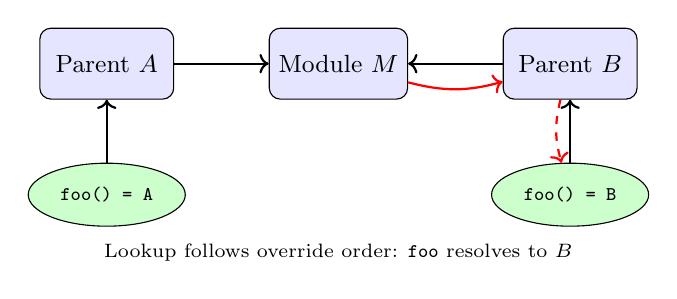
\begin{tikzpicture}[
  node distance=1.2cm and 1.2cm,
  module/.style={rectangle, draw=black, rounded corners, minimum width=1.7cm, minimum height=0.9cm, fill=blue!10, font=\small},
  symbol/.style={ellipse, draw=black, fill=green!20, minimum width=1.4cm, minimum height=0.8cm, font=\scriptsize},
  edge/.style={->, thick},
  rededge/.style={->, thick, red},
  dashededge/.style={->, dashed, thick, gray}
]

% Nodes
\node[module] (M) at (0,0) {Module $M$};
\node[module] (A) [left=of M] {Parent $A$};
\node[module] (B) [right=of M] {Parent $B$};

\node[symbol] (defA) [below=0.8cm of A] {\texttt{foo() = A}};
\node[symbol] (defB) [below=0.8cm of B] {\texttt{foo() = B}};

% Inheritance edges
\draw[edge] (A) -- (M);
\draw[edge] (B) -- (M);

% Definition edges
\draw[edge] (defA) -- (A);
\draw[edge] (defB) -- (B);

% Resolution path
\draw[rededge] (M) to[bend right=15] (B);
\draw[rededge, dashed] (B) to[bend right=15] (defB);

% Optional fallback (commented)
% \draw[dashededge] (B) to[bend left=20] (A);
% \draw[dashededge] (A) to[bend left=20] (defA);

% Legend
\node[align=center, font=\scriptsize] at (0, -2.4) {Lookup follows override order: \texttt{foo} resolves to $B$};

\end{tikzpicture}
\caption{
Symbol resolution in a Merkle-based inheritance graph. Module $M$ inherits from parents $A$ and $B$, with left-to-right override precedence. The red arrows illustrate the path taken to resolve the symbol \texttt{foo}, which is found in $B$. Dotted red arrows represent resolution from the parent to the symbol definition.
}
\label{fig:semantics}
\end{figure}

\section{Namespace-Based Registry}
\label{sec:namespace-based-registry}

To facilitate human-readable and interoperable module references, we introduce a decentralized registry system that maps symbolic names and version constraints to Merkle-based module identities. This registry layer provides a structured namespace for modules while preserving the immutability and transparency of the underlying content-addressed architecture.

\subsection{Human-Readable Naming}

To enable discoverability and developer ergonomics, modules may be referred to by symbolic identifiers of the form:
\[
\texttt{namespace/name@version}
\]

For example:
\[
\texttt{core/math@1.0.0}
\]

These identifiers are resolved to finalized module hashes via a distributed registry system.

\subsection{Registry Semantics}

We define a registry as a mapping:
\[
\mathcal{R}: (\texttt{namespace}, \texttt{name}, \texttt{semver}) \rightarrow h_M
\]

Each registry entry is a triple that maps a human-readable namespace and identifier and a semantic version constraint to a finalized module ID.

\subsection{Version Constraints}

The current system supports only \emph{exact versioning} for modules. Modules must be referenced using fully specified semantic versions, such as \texttt{core/math@1.2.3}

This ensures reproducibility and avoids ambiguity during resolution. Each version corresponds to a finalized module hash, and resolution is a direct lookup of that specific version in the distributed registry.

While this restriction simplifies caching, distribution, and verification, it limits the ability to express flexible or evolving dependencies. As future work, we plan to support more expressive version constraints, including:

\begin{itemize}
    \item Compatible Versions: \verb#@^1.2.0#
    \item Version Ranges: \texttt{>=1.0.0 <2.0.0}
\end{itemize}

These forms would require additional mechanisms for compatibility analysis, deterministic resolution, and finalization tracking across evolving module sets.
\subsection{Support for \texttt{latest} Tag in Module References}

To improve developer ergonomics during early development and testing, the system supports symbolic module references using a reserved \texttt{latest} tag. This tag acts as a placeholder for the most recent version of a module available at the time of resolution, determined using a combination of metadata (e.g., version numbers, timestamps) or registry-specific heuristics.

\paragraph{Pre-Finalization Semantics.}
The \texttt{latest} tag is resolved during the pre-finalization phase of module compilation or bundling. At this stage, all symbolic references are dereferenced to content-addressed identifiers (e.g., hashes), ensuring that the finalized module graph remains immutable and reproducible. This allows developers to write:

\begin{verbatim}
import utils from "example.org/lib@latest";
\end{verbatim}

\noindent which is resolved to:

\begin{verbatim}
import utils from "example.org/lib@1.2#hash";
\end{verbatim}

\noindent based on the state of the distributed registry or a pinned version map at the time of finalization.

\paragraph{Reproducibility and Pinning.}
To ensure builds remain deterministic, the resolution of \texttt{latest} must be pinned to a concrete content hash before module finalization. Once resolved, symbolic tags are no longer part of the module graph. Build systems and registries should retain a record of the mapping between symbolic tags and resolved identifiers to support reproducibility audits.

\paragraph{Limitations.}
Because the \texttt{latest} tag is inherently non-deterministic, its use is discouraged in finalized modules or published registries. It is intended for use in development workflows, rapid prototyping, and interactive environments such as REPLs or notebooks. Static analyzers and linters may issue warnings if \texttt{latest} appears in production code paths.

\paragraph{Related Features.}
The system may also support additional symbolic tags like \texttt{beta}, \texttt{stable}, or semver-compatible wildcards (e.g., \texttt{1.x}), resolved via similar mechanisms before finalization. All symbolic references must ultimately reduce to a content-addressed form to participate in the Merkle tree-based inheritance model.

\subsection{Immutable Bindings}

Once a registry entry is created, it is immutable. That is:
\[
\mathcal{R}(n, m, v) = h_M \quad \text{is fixed for all time}
\]

This ensures that symbolic references remain stable and verifiable over time.

\subsection{Distributed Implementation}

The registry is implemented as a distributed store backed by the same DHT infrastructure used for module exchange~\cite{dht}. Each namespace is a signed collection of bindings, rooted by a Merkle tree~\cite{merkle1978}:
\[
\texttt{namespace} \rightarrow H_{\text{merkle}}(\text{bindings})
\]

Each binding is a tuple:
\[
(\texttt{name}, \texttt{version}, h_M)
\]

Namespaces may be published and updated only by owners who can sign new Merkle roots. Ownership is tracked via public key cryptography, and clients verify signatures before accepting updates.

\subsection{Integration with Finalization}

During module finalization, any symbolic parent reference of the form:
\begin{verbatim}
import core/math@1.0.0
\end{verbatim}
is resolved through the registry:
\[
(\texttt{core}, \texttt{math}, \texttt{1.0.0}) \xrightarrow{\mathcal{R}} h_{M'}
\]

The resulting module ID $h_{M'}$ is inserted into the parent set $P$, and all symbolic names are replaced by cryptographic hashes. This process is deterministic and ensures that the final module ID is fully derived from immutable data.

\subsection{Registry Trust Model}

Registries do not require global trust. Clients are free to:
\begin{itemize}
    \item Pin specific hashes instead of using symbolic names.
    \item Use alternate or private registries for specific namespaces.
    \item Require signatures from known authors or authorities.
\end{itemize}

This flexibility allows the ecosystem to support both centralized and decentralized workflows while preserving verifiability.

\section{Runtime and Resolution Semantics}
\label{sec:runtime-resolution-semantics}

In Tangl, modules are compiled into a platform-independent format (e.g., WebAssembly or JavaScript) and executed in a virtual machine (VM). A finalized module is fully deterministic: it includes a content-addressed identifier, a static resolution table, and a record of its transitive ancestry. At execution time, this structure enables on-demand, verifiable, and reproducible behavior.

\subsection{Resolve Phase}

Rather than preloading all dependencies, the Tangl VM performs a \emph{resolve phase} prior to execution:

\begin{itemize}
    \item It traverses the module’s resolution map $R_M$, which maps symbol names to ancestor modules and specific exports.
    \item For each module ID referenced in $R_M$, it checks whether the corresponding module is available locally or locates it in the distributed network.
    \item A resolution index $\rho: h_{M_i} \mapsto \text{location}$ is constructed, mapping content hashes to their resolvable location (e.g., a local path, cached artifact, or network URI).
\end{itemize}

No modules are actually fetched or loaded during this phase. Instead, the resolve phase ensures that all necessary modules are \textit{locatable}, enabling efficient runtime linking.

\subsection{Lazy Loading at Runtime}

Once resolution is complete, the module is executed with \emph{lazy loading} semantics:

\begin{itemize}
    \item Ancestor modules are not loaded upfront.
    \item When a symbol is first accessed during execution, the VM uses $R_M$ to determine which ancestor module it belongs to.
    \item If the ancestor has not yet been loaded, the VM consults $\rho$ to fetch, parse, and instantiate it on demand.
    \item Resolved exports are cached for subsequent use.
\end{itemize}

This strategy ensures minimal startup overhead, efficient caching, and deterministic behavior across environments.


\subsection{Symbol Resolution Example}

To illustrate the resolution logic, consider a module \texttt{Main} that inherits from two modules \texttt{A} and \texttt{B}, both of which export a symbol \texttt{foo}. Tangl's resolution map $R_M$ determines which export is used based on two factors:

\begin{itemize}
    \item \textbf{Import Order:} If both modules define the same symbol, the last one imported "wins" by default.
    \item \textbf{Import Granularity:} A symbol-specific import (e.g., \texttt{import(A.foo)}) takes precedence over whole-module imports.
\end{itemize}

\paragraph{Scenario 1: Whole-module imports, ordered B then A}

\begin{verbatim}
import(B);
import(A);
foo();
\end{verbatim}

Even though both \texttt{A} and \texttt{B} export \texttt{foo}, the reference map $R_{\texttt{Main}}$ resolves:

\[
R_{\texttt{Main}}(\texttt{foo}) = \langle \texttt{A}, \texttt{foo} \rangle
\]

because \texttt{A} was imported after \texttt{B}, overriding its binding.

\paragraph{Scenario 2: Symbol-specific import.}

\begin{verbatim}
import(A.foo);
import(B);
foo();
\end{verbatim}

Even though \texttt{B} was imported later, the reference map gives priority to the symbol-specific import:

\[
R_{\texttt{Main}}(\texttt{foo}) = \langle \texttt{A}, \texttt{foo} \rangle
\]

This allows developers to explicitly pin symbols to particular modules, regardless of the overall import order.

\paragraph{Scenario 3: No disambiguation provided.}

\begin{verbatim}
import(A);
import(B);
foo();
\end{verbatim}

This resolves to:

\[
R_{\texttt{Main}}(\texttt{foo}) = \langle \texttt{B}, \texttt{foo} \rangle
\]

since \texttt{B} was the last module imported that provided \texttt{foo}. Had both modules been imported in the reverse order, the binding would change.

\paragraph{Summary.}

Tangl's resolution rules provide both predictability and flexibility:

\begin{itemize}
    \item The default rule is \textit{last-imported wins}.
    \item Symbol-specific imports override full-module imports.
    \item Resolution is captured statically in $R_M$, which is persisted in the finalization step and guarantees reproducibility across machines and time.
\end{itemize}

This allows Tangl programs to explicitly disambiguate conflicting definitions and avoid ambiguous resolution paths without resorting to runtime heuristics.

\begin{lstlisting}[language=Python,
    caption={Lazy symbol resolution in the \texttt{Resolver} class},
    label={fig:lazy-resolution},
    basicstyle=\scriptsize\ttfamily,
    breaklines=true,
    breakindent=0pt,
    frame=single,
    columns=fullflexible,
    keepspaces=true
]
class Resolver:
    def __init__(self, reference_map, content_store, fetch_from_network):
        self.reference_map = reference_map  # {'foo': 'hash123'}
        self.cs = content_store             # Local content store
        self.fetch = fetch_from_network     # Fetch fn
        self.resolved_cache = {}            # Memoized resolutions

    def resolve(self, symbol):
        if symbol in self.resolved_cache:
            return self.resolved_cache[symbol]
        if symbol not in self.reference_map:
            raise ResolutionError(f"Symbol {symbol} not found")
        hash_id = self.reference_map[symbol]
        if not self.cs.contains(hash_id):
            module_data = self.fetch(hash_id)
            self.cs.store(hash_id, module_data)
        module = self.cs.load(hash_id)
        self.resolved_cache[symbol] = module
        return module

resolver = Resolver(reference_map, content_store, network_fetch_fn)
foo_module = resolver.resolve('foo')
\end{lstlisting}

\begin{figure}[ht]
\centering
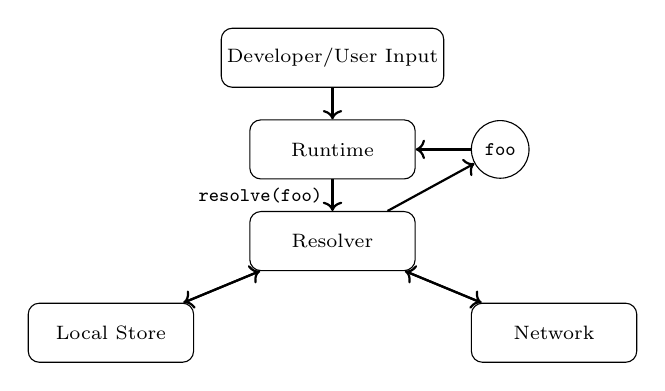
\begin{tikzpicture}[
  node distance=4mm and 7mm,
  font=\scriptsize,
  box/.style={draw, rounded corners, align=center, minimum width=2.1cm, minimum height=0.75cm, inner sep=2pt},
  arrow/.style={->, thick},
  sym/.style={circle, draw, minimum size=0.7cm, align=center}
]

% Nodes
\node[box] (dev) {Developer/User Input};
\node[box, below=of dev] (runtime) {Runtime};
\node[sym, right=of runtime] (foo) {\texttt{foo}};
\node[box, below=of runtime] (resolver) {Resolver};
\node[box, below left=of resolver] (local) {Local Store};
\node[box, below right=of resolver] (network) {Network};

% Edges
\draw[arrow] (dev) -- (runtime);
\draw[arrow] (runtime) -- (resolver) node[midway, left] {\texttt{resolve(foo)}};
\draw[arrow] (resolver) -- (local);
\draw[arrow] (resolver) -- (network);
\draw[arrow] (local) -- (resolver);
\draw[arrow] (network) -- (resolver);
\draw[arrow] (resolver) -- (foo);
\draw[arrow] (foo) -- (runtime);

\end{tikzpicture}
\caption{Runtime resolution of symbols like \texttt{foo} through local or network lookup.}
\label{fig:interactive-resolution}
\end{figure}

\subsection{Module Resolution Walkthrough}

To illustrate the module resolution process and how conflicts are handled, consider the following scenario involving two modules, \texttt{moduleA} and \texttt{moduleB}, both of which define a function \texttt{compute()}:

\begin{verbatim}
# moduleA.js
export function compute() { return 42; }

# moduleB.js
export function compute() { return 24; }
\end{verbatim}

A third module, \texttt{moduleC}, imports both \texttt{moduleA} and \texttt{moduleB}, and then calls \texttt{compute()}:

\begin{verbatim}
# moduleC.js
import { compute } from 'moduleA';
import { compute } from 'moduleB';

console.log(compute());
\end{verbatim}

Module resolution begins by evaluating imports in lexical order. In this case, the function \texttt{compute} from \texttt{moduleB} shadows the one from \texttt{moduleA} because it is imported later. Thus, \texttt{console.log(compute())} prints \texttt{24}, not \texttt{42}.

This rule, where later imports take precedence, is a key aspect of the system’s lexical scoping model and ensures predictability: the most recently imported binding of a symbol is the one used.

\paragraph{Re-Exports.}

Now consider a re-export scenario where a module re-exports symbols from another:

\begin{verbatim}
# moduleA.js
export function compute() { return 42; }

# moduleB.js
export { compute } from 'moduleA';
export function compute() { return 24; }

# moduleC.js
import { compute } from 'moduleB';
console.log(compute());
\end{verbatim}

Here, \texttt{moduleB} re-exports \texttt{compute} from \texttt{moduleA}, but also defines its own version of \texttt{compute}. The local definition in \texttt{moduleB} takes precedence over the re-exported one, and so \texttt{console.log(compute())} prints \texttt{24}.

\paragraph{Nested Imports.}

Finally, consider a case with nested imports:

\begin{verbatim}
# base.js
export function compute() { return 1; }

# lib.js
import { compute as baseCompute } from 'base';
export function compute() {
    return baseCompute() + 1;
}

# app.js
import { compute } from 'lib';
console.log(compute());
\end{verbatim}

In this example, \texttt{lib.js} imports \texttt{compute} from \\\texttt{base.js} under the alias \texttt{baseCompute}, then defines its own \texttt{compute} that builds on it. When \texttt{app.js} imports from \texttt{lib.js}, it sees only the final \texttt{compute}—which returns \texttt{2}.

This demonstrates how symbol resolution in nested modules always respects lexical ordering and explicit rebinding: imported symbols are only visible where they are explicitly propagated.

\paragraph{Summary.}

These examples collectively illustrate how lexical import order and explicit rebindings guide name resolution. The "last import wins" rule ensures intuitive behavior while allowing developers to override or refine imported symbols as needed.

\subsection{Execution Model Summary}

Execution proceeds as follows:
\begin{enumerate}
    \item \textbf{Resolve:} Traverse $R_M$ to locate all ancestor modules by hash and build $\rho$.
    \item \textbf{Instantiate:} Load and prepare \texttt{Main} for execution with no parent modules yet loaded.
    \item \textbf{Evaluate:} As symbols are accessed, dynamically load ancestors and resolve symbols according to $R_M$.
\end{enumerate}

This model allows large dependency graphs to be traversed efficiently and on-demand, while maintaining strong guarantees of determinism, immutability, and verifiability.

\begin{figure*}[ht]
\centering
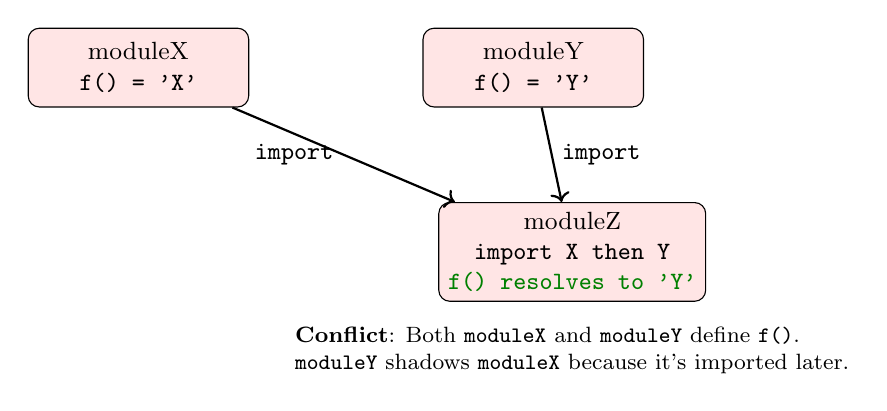
\begin{tikzpicture}[
  node distance=1.7cm and 2.2cm,
  every node/.style={font=\small},
  module/.style={rectangle, draw=black, fill=red!10, rounded corners, minimum width=2.8cm, minimum height=1cm, align=center},
  arrow/.style={->, thick}
]

% Modules for Conflict Scenario
\node[module] (modX) {moduleX\\ \texttt{f() = 'X'}};
\node[module, right=of modX] (modY) {moduleY\\ \texttt{f() = 'Y'}};
\node[module, below right=1.2cm and 2.4cm of modX] (modZ) {moduleZ\\ \texttt{import X then Y}\\ \texttt{\textcolor{green!50!black}{f() resolves to 'Y'}}};

% Arrows for Conflict Scenario
\draw[arrow] (modX) -- (modZ) node[midway, left] {\texttt{import}};
\draw[arrow] (modY) -- (modZ) node[midway, right] {\texttt{import}};

% Annotation for Conflict Scenario
\node[align=left, below=0.2cm of modZ, font=\footnotesize] {
\textbf{Conflict}: Both \texttt{moduleX} and \texttt{moduleY} define \texttt{f()}.\\
\texttt{moduleY} shadows \texttt{moduleX} because it's imported later.
};

\end{tikzpicture}

\vspace{1cm}  % Add some space between the two diagrams

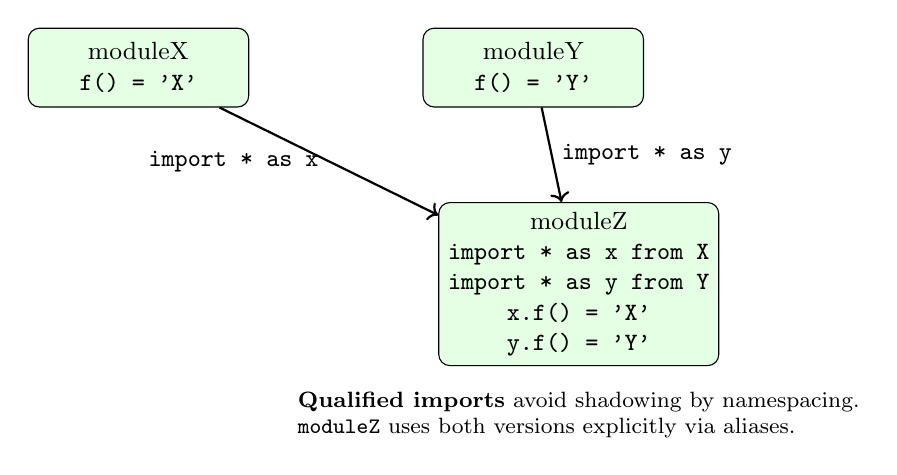
\begin{tikzpicture}[
  node distance=1.7cm and 2.2cm,
  every node/.style={font=\small},
  module/.style={rectangle, draw=black, fill=green!10, rounded corners, minimum width=2.8cm, minimum height=1cm, align=center},
  arrow/.style={->, thick}
]

% Modules for Qualified Import Scenario
\node[module] (modX) {moduleX\\ \texttt{f() = 'X'}};
\node[module, right=of modX] (modY) {moduleY\\ \texttt{f() = 'Y'}};
\node[module, below right=1.2cm and 2.4cm of modX] (modZ) {moduleZ\\ \texttt{import * as x from X}\\ \texttt{import * as y from Y}\\ \texttt{x.f() = 'X'}\\ \texttt{y.f() = 'Y'}};

% Arrows for Qualified Import Scenario
\draw[arrow] (modX) -- (modZ) node[midway, left] {\texttt{import * as x}};
\draw[arrow] (modY) -- (modZ) node[midway, right] {\texttt{import * as y}};

% Annotation for Qualified Import Scenario
\node[align=left, below=0.2cm of modZ, font=\footnotesize] {
\textbf{Qualified imports} avoid shadowing by namespacing.\\
\texttt{moduleZ} uses both versions explicitly via aliases.
};

\end{tikzpicture}

\vspace{1cm}  % Add some space between the two diagrams

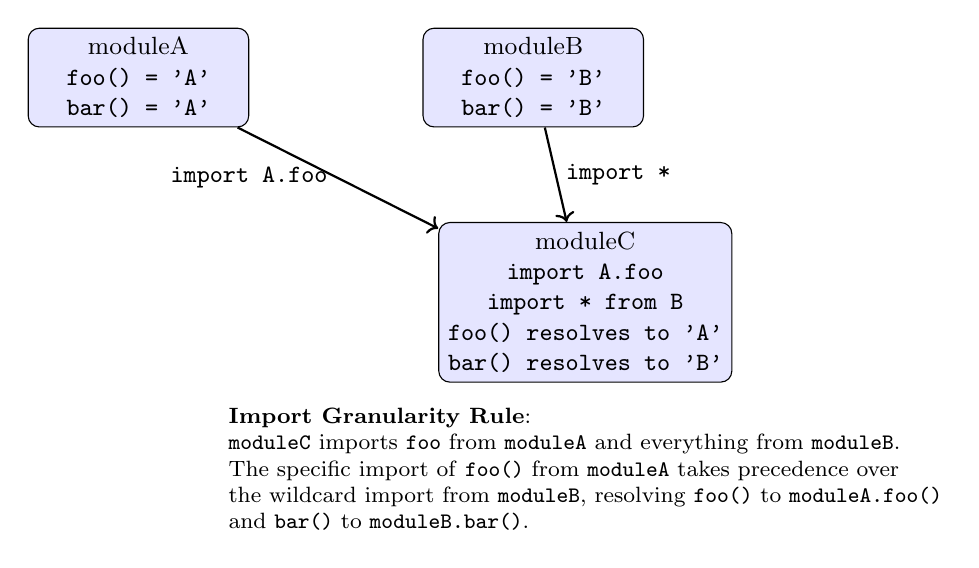
\begin{tikzpicture}[
  node distance=1.7cm and 2.2cm,
  every node/.style={font=\small},
  module/.style={rectangle, draw=black, fill=blue!10, rounded corners, minimum width=2.8cm, minimum height=1cm, align=center},
  arrow/.style={->, thick}
]

% Modules for New Scenario (A imports foo, B imports foo & bar)
\node[module] (modA) {moduleA\\ \texttt{foo() = 'A'}\\ \texttt{bar() = 'A'}};
\node[module, right=of modA] (modB) {moduleB\\ \texttt{foo() = 'B'}\\ \texttt{bar() = 'B'}};
\node[module, below right=1.2cm and 2.4cm of modA] (modC) {moduleC\\ \texttt{import A.foo}\\ \texttt{import * from B}\\ \texttt{foo() resolves to 'A'}\\ \texttt{bar() resolves to 'B'}};

% Arrows for New Scenario
\draw[arrow] (modA) -- (modC) node[midway, left] {\texttt{import A.foo}};
\draw[arrow] (modB) -- (modC) node[midway, right] {\texttt{import *}};

% Annotation for New Scenario
\node[align=left, below=0.2cm of modC, font=\footnotesize] {
\textbf{Import Granularity Rule}:\\
\texttt{moduleC} imports \texttt{foo} from \texttt{moduleA} and everything from \texttt{moduleB}.\\
The specific import of \texttt{foo()} from \texttt{moduleA} takes precedence over\\
the wildcard import from \texttt{moduleB}, resolving \texttt{foo()} to \texttt{moduleA.foo()}\\
and \texttt{bar()} to \texttt{moduleB.bar()}.
};

\end{tikzpicture}

\vspace{1cm}  % Add some space between the two diagrams

\caption{Module resolution: (a) Conflict resolution with lexical shadowing, where the last import wins. (b) Qualified imports preserve access to all symbols without shadowing by using aliases. (c) Demonstrating the import granularity rule: a specific import of \texttt{foo} from \texttt{moduleA} takes precedence over the general import of everything from \texttt{moduleB}, resolving \texttt{foo()} to \texttt{moduleA.foo()} and \texttt{bar()} to \texttt{moduleB.bar()}.}
\label{fig:module-resolution}
\end{figure*}

\subsection{Incremental Inheritance and Differential Reuse}
\label{sec:overlays}

In immutable, content-addressed module systems, every module is identified by a cryptographic hash of its contents. This immutability provides strong guarantees—such as referential transparency, verifiable caching, and decentralized fetch—but it also presents challenges when incremental updates or overrides are needed.

Rather than allowing in-place mutation or overlays, such systems promote \emph{differential reuse} through fine-grained modularization. Reusable logic is factored into small, composable units that can be selectively inherited and extended. When a change is necessary, a new module imports one or more ancestors and extends or overrides their contents, producing a new hash and a new node in the inheritance tree.

These systems are typically language-agnostic, deferring to the host language or runtime to resolve overlapping definitions. Resolution is often governed by a deterministic traversal of the module ancestry graph, such as a topological sort of the Merkle DAG, possibly ordered lexicographically by content hash.

This approach parallels strategies in existing systems: Git commits form immutable DAGs that track content evolution;\footnote{Git's object model ensures immutability and deduplication via SHA-1/SHA-256 content hashes, enabling reproducible version histories.} Nix builds use content-addressed derivations and dependency graphs to isolate and reproduce environments;\footnote{The Nix package manager treats software builds as pure functions, with inputs hashed to ensure deterministic outputs and maximal reuse.} and IPFS organizes files in Merkle DAGs to enable decentralized sharing and incremental updates.\footnote{IPFS (InterPlanetary File System) encodes file versions and directories as Merkle trees, allowing deduplicated and verifiable content exchange.} Promoting fine-grained modularization discourages monolithic library modules in favor of small, single-purpose modules that can be easily transmitted and executed on all manner of host configurations.

Future extensions may explore support for semantic diffs, patch modules, or structured deltas. These approaches could reduce duplication in the module graph, improve resolution performance, and allow for more expressive forms of inheritance without compromising immutability or verifiability.

\section{Optimizations and Caching}
\label{sec:optimizations}

The modular resolution model presented in this paper supports a variety of optimizations that improve both runtime performance and network efficiency, while preserving the determinism and compositionality of the system.

The primary opportunity for optimization lies in the \textit{resolve phase}, during which symbolic references are matched against entries in the reference map and resolved to content-addressed identifiers. Because resolution is deterministic and purely functional with respect to the reference graph, the results of this phase can be cached and reused across executions, contexts, and even deployments.

To support efficient execution, the system defers the fetching and linking of modules until they are actually needed, enabling a form of \textit{lazy loading}. Rather than eagerly loading the full transitive closure of a program's dependencies, the runtime can locate only those modules that are necessary for the execution of a given entry point. This is particularly effective in large module hierarchies or interactive environments, where only a subset of bindings are used in a given session.

The reference graph itself is well-suited to caching, both locally and in networked deployments. Because every node in the graph is identified by a content hash, any resolved module can be safely cached without risk of inconsistency. In distributed settings, resolved modules can be fetched from nearby peers or mirrors, with trust rooted in the immutability of the content hash. This allows for efficient and resilient retrieval of modules without the need for centralized coordination or a trusted registry.

Symbol resolution is further optimized by exploiting structural properties of the reference map. For example, when a symbol is requested, the runtime can avoid unnecessary traversals by using a scoped cache of previously resolved bindings. Because resolution follows a lexically-scoped and shadowing-aware order, these bindings can be reused for subsequent queries in the same context.

Overall, the caching and lazy resolution strategy supports rapid execution, offline availability, and scalable distribution without compromising the reproducibility or auditability of the resulting execution. The modular and immutable nature of the reference graph allows these optimizations to be layered on top of the formal resolution semantics, rather than requiring changes to the resolution model itself.

\subsection{Scalability of Cryptographic Mechanisms}
\label{sec:scalability-crypto}

While Merkle tree-based inheritance offers strong guarantees of immutability, integrity, and reproducibility, it also introduces computational overhead when applied to large module graphs. In large-scale ecosystems, the transitive ancestry of a module may span tens or hundreds of thousands of modules, each contributing to the final Merkle root.

To mitigate this cost, our system implements subtree memoization and batched ancestry hashing. Rather than recomputing the entire tree on every resolution, previously computed subtrees are cached and reused whenever their structure remains unchanged. This significantly reduces both CPU overhead and memory consumption during finalization.

Hash computation is structured as a bottom-up traversal of the module DAG, enabling parallelization across subtrees. This design integrates naturally with distributed build systems and continuous integration pipelines, where isolated subgraphs can be finalized independently and reused across builds.

Importantly, finalized modules are immutable. Their Merkle subtrees can be shared across dependents without duplication, enabling efficient reuse and dramatically reducing redundant hashing. In large registries, this reuse leads to logarithmic rather than linear growth in unique hash entries.

Future extensions may incorporate authenticated data structures, such as vector commitments or sparse Merkle trees, to compress ancestry proofs and further reduce tree depth, particularly for flat or highly reused module hierarchies.

\section{Developer Tooling}
\label{sec:developer-tooling}

A module system grounded in Merkle tree-based inheritance and content-addressed resolution introduces new interaction models for developers. This section outlines the types of tools and developer experiences needed to work effectively with such a system, especially as module graphs grow in size and complexity.

\subsection{Module Graph Visualization}

Inheritance and dependency graphs in Merkle-based systems can grow large and complex, particularly with deep chains of module reuse or broad forks in ancestry. Developer tooling should support interactive graph visualizations, showing both lexical import structure and resolved ancestry. This helps identify where symbols originate, which modules are shadowed, and how resolution paths are computed. Tools should allow filtering by symbol, version, or ancestry to pinpoint specific resolution behaviors.

\subsection{Error Reporting and Diagnostics}

When resolution fails, due to missing modules, unresolved identifiers, or hash mismatches, the system should provide rich diagnostics:
\begin{itemize}
  \item Symbol resolution traces showing candidate paths and overrides.
  \item Hash mismatch explanations with expected vs. actual content.
  \item Resolution conflicts with suggestions for disambiguation.
\end{itemize}

Because modules are immutable, ancestry traces are often more informative than runtime stack traces. Tooling should simulate step-by-step resolution paths to clarify precedence and shadowing.

\subsection{IDE and CLI Integration}

Integration with modern IDEs and CLI environments is critical. Features include:

\begin{itemize}
  \item Auto-completion for inherited symbols and re-exports.
  \item Hover-based ancestry and override inspection.
  \item Inline diffs between overridden definitions.
  \item Symbol provenance queries via CLI.
  \item Dry-run simulations of finalization and resolution behavior.
\end{itemize}

Tooling integrates with VS Code, JetBrains IDEs, and common shells, exposing both real-time editing support and CI/CD debugging aids.

\begin{figure}[ht]
\centering
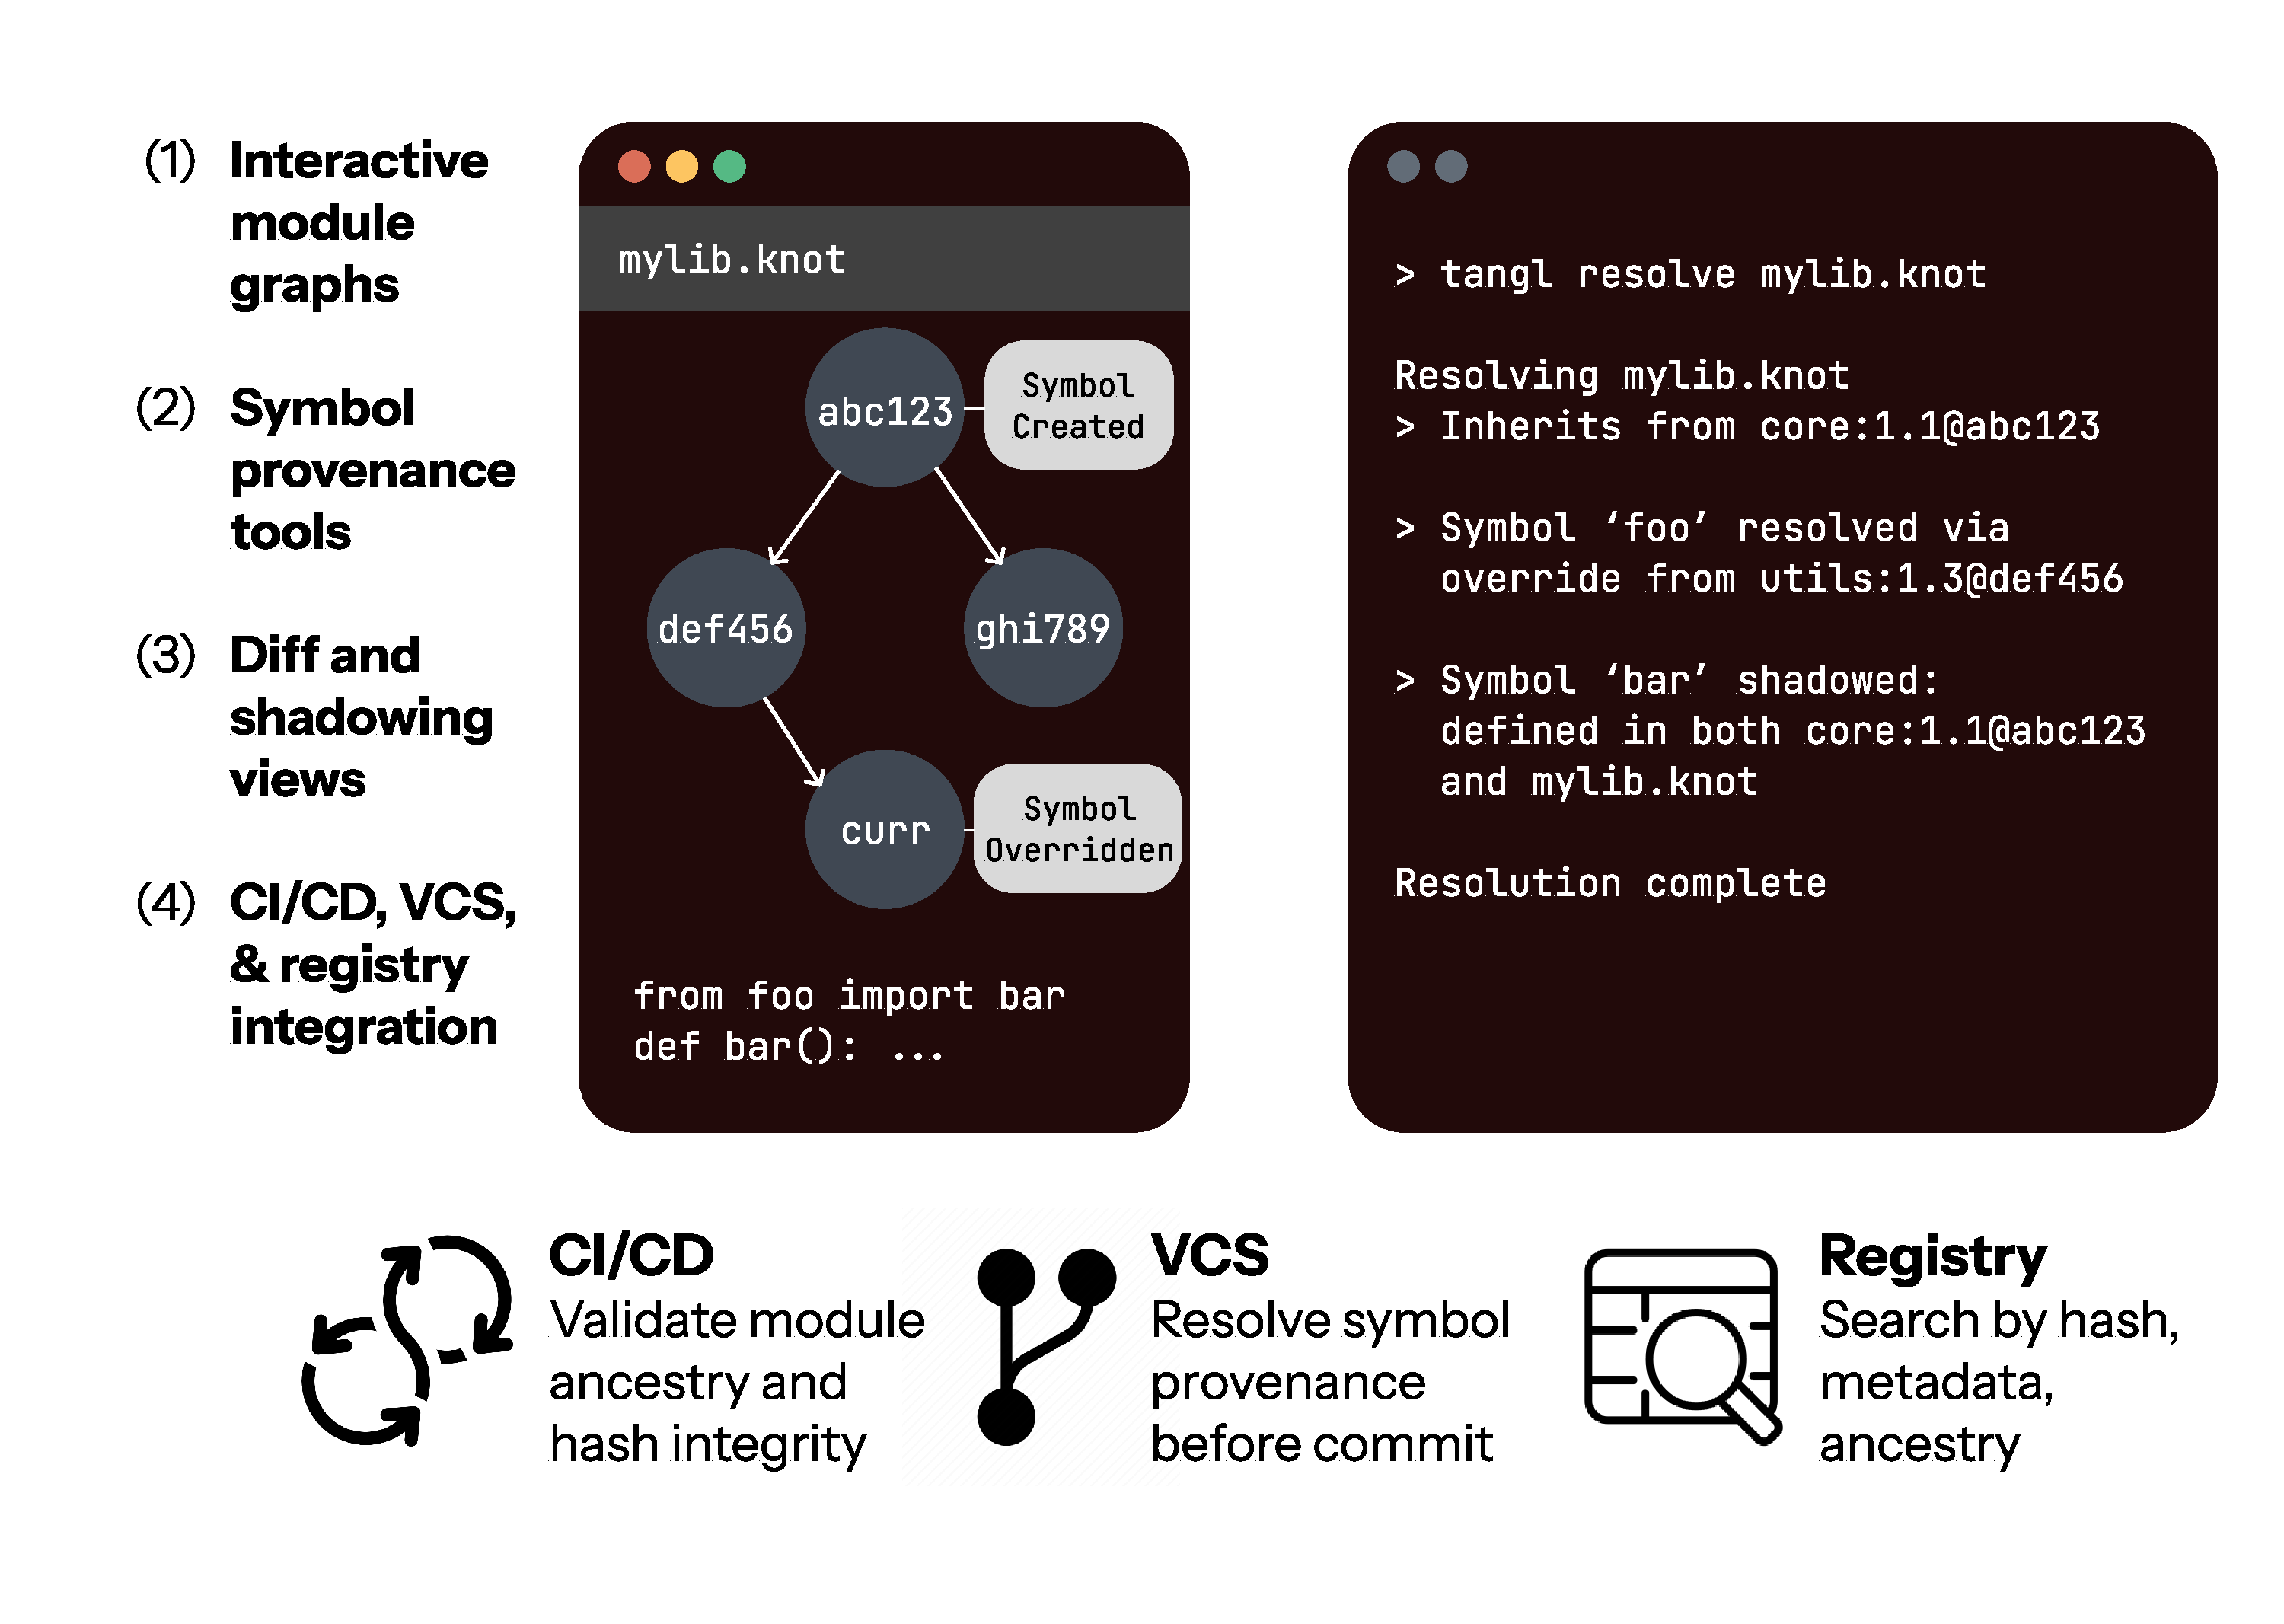
\includegraphics[width=\linewidth]{merkle_inheritance_ux.pdf}
\caption{
A conceptual overview of developer tooling for Merkle-based module systems. IDE and CLI tools provide layered insights: (1) interactive module graphs show lexical and resolved ancestry; (2) symbol provenance tools trace resolution across override chains; (3) diff and shadowing views visualize active vs overridden definitions; and (4) integration with CI/CD, VCS, and registries supports reproducibility and ecosystem interoperability.
}
\label{fig:tooling}
\end{figure}

\subsection{Debugging Overridden Definitions}

Given the potential for deep inheritance chains and override conflicts, tools should help developers reason about which definitions are active, which are overridden, and why. Especially in the presence of complex MRO-like resolution orders, IDEs or visualization layers should explain precedence and substitution clearly. Symbol diff tools, shadowing inspectors, and override explainers can improve transparency and prevent subtle bugs due to unexpected overrides.

\subsection{Visual Tooling for Symbol Overrides and Ancestry Tracing}
\label{sec:tooling-visuals}

Consider a scenario where a developer hovers over a symbol like \texttt{foo()} in an IDE. The tooling might display:

\begin{itemize}
  \item The Merkle root or alias of the module where \texttt{foo()} was defined,
  \item A linear ancestry of overrides (\texttt{moduleA} $\rightarrow$ \texttt{moduleB} $\rightarrow$ \texttt{current}),
  \item Inline diffs for each override.
\end{itemize}

\begin{lstlisting}[language=, caption={Mockup of a symbol override trace as presented in an IDE}, label={lst:override_trace_mockup}, basicstyle=\ttfamily\small]
[Trace] Symbol: foo()
Resolved to:
  moduleC@b17e... (current context)
Override history:
  - moduleC@b17e...
    -> override of foo() [defined inline]
  - moduleB@a9c4...
    -> re-exported from moduleA@d3e1...
  - moduleA@d3e1...
    -> original definition:
       function foo() { return 42; }
Ancestry path:
  moduleA -> moduleB -> moduleC
[OK] This symbol was overridden in moduleC
[INFO] Click to view diff between 
    moduleC::foo and moduleA::foo
\end{lstlisting}

\subsection{Best Practices and Developer Guidance}
\label{sec:best-practices}

To ensure predictable and maintainable behavior, developers should adhere to the following practices:

\paragraph{Avoid Unintentional Shadowing:} Since symbol resolution follows a deterministic merge order, avoid shadowing an imported symbol unless intentionally overriding the logic for that symbol.

\paragraph{Use Explicit Imports for Critical Symbols:} Prefer explicit imports of key symbols when re-exporting from deeply nested modules. \texttt{import(a.foo)} is better than \texttt{import(a)} if you only need to access \texttt{foo}.

\paragraph{Pin Modules Before Finalization:} Always resolve imports to content hashes as soon as you know what functionality you need. This prevents unexpected behavior from the \texttt{latest} tag as new modules are uploaded. 

\paragraph{Document Inheritance Chains:} Document override purposes and expected resolution behaviors. This aids in both auditing and usage of your code.

\paragraph{Validate Resolution with Tooling:} Use diagnostics and linters to confirm that resolution paths are deterministic.

\paragraph{Prefer Compositional Reuse:} Shallow hierarchies simplify debugging and reduce resolution cost. Prefer direct imports over indirect ones, when possible.

\section{Ecosystem Integration and Usability}
\label{sec:ecosystem}

Usability at scale depends not only on local developer tooling but also on system-level integration. This section discusses how Merkle-based modules interact with package managers, CI/CD workflows, and registries.

\subsection{Integration with Existing Package Managers}

The system is designed to interoperate with existing build and package management ecosystems. Compatibility tools can be created to allow developers to continue using \texttt{npm}, \texttt{Cargo}, or \texttt{pip} while gaining immutability and content-based resolution.

\begin{itemize}
  \item \texttt{npm merkle-resolve} would add content hash locking to \texttt{package.json}.
  \item \texttt{cargo finalize} would validate dependency graphs before publishing.
  \item \texttt{pip-merk} would overlay Merkle-tracked modules into virtual environments.
  \item etc.
\end{itemize}

These integrations ensure a gradual adoption path for existing codebases.

\subsection{Community and Ecosystem Tooling}

As module systems grow beyond individual projects, ecosystem-facing tools become essential:
\begin{itemize}
  \item Search by hash prefix, semantic version, or ancestry similarity.
  \item Provenance visualization and diffing between forks.
  \item Module discovery through public or federated registries.
  \item Moderated publication pipelines for namespaces and groups.
\end{itemize}

Registry APIs expose reproducibility guarantees and ancestry-based filtering, allowing deeper insights into module evolution.

\subsection{UI Affordances and Developer Trust}

Cryptographic guarantees are necessary but not sufficient. Tools should also surface human-readable trust signals:

\begin{itemize}
  \item Verified authorship (e.g., PGP signatures or decentralized IDs).
  \item Maintainer metadata and reputation indicators.
  \item Visualized module forks and merge histories.
  \item Attestations of build reproduction or CI checks.
\end{itemize}

These affordances help developers navigate decentralized module ecosystems with greater confidence.

\subsection{End-User Trust and UI Affordances}
\label{sec:trust-ui}

In decentralized systems where module resolution depends on transitive ancestry, trust becomes not only a cryptographic but also a human-comprehensible property. To make the Merkle-based model approachable for developers, we outline several affordances and UX principles for building trust and transparency into tooling.

\paragraph{Visualizing Ancestry and Inheritance.}
Graphical interfaces should render inheritance hierarchies as DAGs with clear origin points, version labels, and shadowing relationships. By allowing users to inspect a module’s full ancestry—down to the hash of each contributing node—tools can make otherwise opaque resolution behaviors auditable and explainable. UI elements such as hover-to-expand ancestry and click-to-trace symbol origin would help users verify correctness and trace override behavior.

\paragraph{Conflict and Shadowing Feedback.}
In cases where symbols are shadowed, redefined, or inherited from conflicting sources, IDEs and CLI tools should surface this information through precise diagnostics. For example, a redefinition should include a warning with the hash and origin of the overshadowed definition, allowing users to distinguish intentional overrides from accidental conflicts.

\paragraph{Provenance and Content Integrity.}
Since all modules are content-addressed, the system guarantees immutability and integrity. To leverage this at the user level, we propose visual markers (e.g., lock icons, color-coded trust levels) indicating whether a module has a known provenance (e.g., signed by a trusted party, linked to a public repository) or is anonymously authored. This also supports audit logs and reproducibility for CI/CD workflows.

\paragraph{Resolution Preview and Explainability.}
Before committing to a resolution (e.g., during installation or CI runs), tools should offer a dry-run or preview mode that shows the exact resolved graph, ancestry paths, and expected runtime behavior. This preemptively catches surprises and builds confidence in the decentralized resolution logic.

\paragraph{Fallback and Error Diagnosis.}
If a resolution fails, due to unavailability, conflict, or missing parents, the UI should provide a structured diagnosis: which hash or module could not be fetched, what the fallback path was, and what resolution rule was violated. These diagnostics reinforce the explainability of resolution semantics and empower users to act on failure cases without guessing.

\paragraph{Distributed Trust as a Design Goal.}
Ultimately, the decentralized nature of the system allows users to define their own trust policies: whether to trust modules from known domains, require signatures from specific keys, or enforce reproducible builds. The user interface should expose these policies transparently and allow users to override, escalate, or audit as needed.

\subsection{Trust, Transparency, and Developer Experience}
\label{sec:trust-ux}

To promote transparency and end-user trust in decentralized module systems, we propose several user interface (UI) and user experience (UX) affordances that make module ancestry, versioning, and resolution behaviors visible and auditable.

\paragraph{Human-Readable Provenance.}
Every module should expose a navigable ancestry tree derived from its Merkle DAG, displaying inherited modules, shadowed symbols, and override boundaries. This supports debugging and helps developers audit the provenance of imported behavior.

\paragraph{Version Pinning Visualizations.}
In interfaces such as IDEs or web registries, developers should be able to inspect which module versions were finalized, whether exact content hashes or semantic ranges were used, and when hash mismatches are detected due to upstream updates.

\paragraph{Ancestry Conflict Warnings.}
When multiple inherited modules define the same symbol (e.g., via diamond inheritance or multi-parent links), IDEs and command-line tools should emit warnings or previews showing which definition will be resolved, under what rule (e.g., left-to-right linearization), and where ambiguity might arise.

\paragraph{Transparency in Hash-Based Locking.}
To reinforce the integrity guarantees of Merkle-based resolution, tooling should surface which parts of a project are hash-locked, which are open to resolution, and which inherit their lock status from parent modules. This allows users to audit potential supply chain risks at resolution time.

\paragraph{Diff and Override Inspection.}
For any module derived from one or more parents, developers should be able to diff the inherited and modified contents. This capability helps identify whether a derived module introduces functional changes, or simply re-exports behavior from its lineage.

\paragraph{Registry and Peer Provenance.}
In decentralized contexts, trust also depends on the source of modules. Tools should display metadata about which registry or peer contributed each resolved module, along with verification of its hash and ancestry. This reduces trust assumptions and helps detect impersonation or mispublishing.

These affordances are critical for developer confidence in decentralized and inheritance-based systems. While the underlying resolution machinery is content-addressed and formally sound, user interfaces must make this machinery explainable and traceable for real-world adoption.

\begin{figure}[ht]
  \centering
  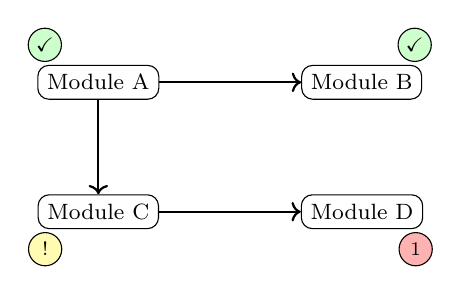
\begin{tikzpicture}[
      module/.style={rectangle, draw=black, rounded corners, minimum height=1.2em, minimum width=3em, align=center, font=\footnotesize},
      trust/.style={circle, draw=black, fill=green!20, inner sep=1pt, font=\scriptsize, minimum width=1.2em},
      warn/.style={circle, draw=black, fill=yellow!30, inner sep=1pt, font=\scriptsize, minimum width=1.2em},
      danger/.style={circle, draw=black, fill=red!30, inner sep=1pt, font=\scriptsize, minimum width=1.2em},
      edge/.style={->, thick},
    ]

    % Nodes
    \node[module] (A) {Module A};
    \node[module, right=1.8cm of A] (B) {Module B};
    \node[module, below=1.2cm of A] (C) {Module C};
    \node[module, right=1.8cm of C] (D) {Module D};

    % Trust indicators
    \node[trust, above left=0.1cm and -0.25cm of A] (TA) {\checkmark};
    \node[trust, above right=0.1cm and -0.25cm of B] (TB) {\checkmark};
    \node[warn, below left=0.1cm and -0.25cm of C] (TC) {!};
    \node[danger, below right=0.1cm and -0.25cm of D] (TD) {{\fontencoding{U}\fontfamily{futs}\selectfont\char 49\relax}};

    % Edges
    \draw[edge] (A) -- (B);
    \draw[edge] (A) -- (C);
    \draw[edge] (C) -- (D);

  \end{tikzpicture}
  \caption{A trust overlay on the module graph. }
  \medskip
  \small
  Each node represents a module, annotated with a trust indicator: green check for verified maintainers, yellow exclamation for unsigned modules, and red warning for known issues or missing signatures. This overlay aids users in evaluating dependency trustworthiness.
  \label{fig:trust-overlay}
\end{figure}

\subsection{Ecosystem Compatibility and Developer Trust}

Maintaining compatibility with existing systems also helps build trust. Developers are more likely to adopt new infrastructure if it complements their existing tooling and requires minimal disruption. This includes supporting familiar metadata formats, dependency declarations, and tooling conventions. Moreover, reproducibility guarantees provided by content-addressed modules can enhance security and build integrity in existing workflows.

\section{Integration with Existing Ecosystems}

While content-addressed, Merkle-based module systems offer significant advantages in immutability, caching, and reproducibility, integration with existing language and package ecosystems remains a key challenge. Developers rarely adopt systems in isolation; instead, they require interoperability with current tools, workflows, and dependency managers.

\subsection{Migration Strategies and Tooling for Legacy Codebases} \label{sec:migration}

To support gradual migration from semver-based systems, our approach uses bridge layers that interpret legacy version constraints (e.g., \verb#"foo": "^1.3.0"#) and resolve them to concrete versions using the host ecosystem’s native resolver (e.g., \texttt{npm}, \texttt{Cargo}). The resulting version (e.g., \texttt{1.3.5}) is then compared against the registry to map it to a finalized Merkle root.

If the registry contains a matching resolution, the import is replaced with the corresponding content hash. If no match is found, the system can fall back to the traditional package manager to fetch and hash the package, optionally storing the result as a new entry in the registry for future use. This preserves deterministic resolution while allowing continued use of familiar semver workflows.

The registry thus acts as a shared, verifiable mirror of resolved legacy imports, ensuring consistent results across machines. Over time, as more packages are pinned and published, projects can transition away from semver without losing reproducibility or compatibility.

Migration tooling can support this process with: 
\begin{itemize} 
  \item \textbf{Bridge-assisted diffing}: Detecting changes between local graphs and published Merkle mappings. 
  \item \textbf{Semantic hashing}: Converting legacy packages into content-addressed modules with symbol-pres-erving boundaries. 
  \item \textbf{Dry-run simulations}: Previewing how semver imports will resolve under Merkle semantics. 
\end{itemize}

This strategy supports incremental adoption without disrupting existing toolchains, while gradually shifting dependency resolution to a globally verifiable, content-addressed model.

\subsection{Incremental Migration Patterns}
\label{sec:incremental-migration}

Migration to a content-addressed module system does not require an all-at-once rewrite. Instead, the system is intentionally designed to support incremental adoption, allowing teams to modernize codebases progressively without disrupting existing workflows.

A common entry point is at the leaf level of the dependency graph, where individual modules can be finalized and published to the registry using content-addressed identities. These leaf modules can be internal libraries, stable third-party packages, or isolated utilities. Because finalization is local and does not require upstream coordination, teams can begin by wrapping existing modules in Merkle-resolved snapshots and registering them for future reuse.

Once these foundational components are finalized, their consumers can migrate independently by switching from semver-based imports to Merkle-resolved references. This process does not require modifying the source logic of the consuming modules, as the registry ensures compatibility and immutability. The result is a smooth transition path in which reproducibility benefits accrue naturally as more modules opt into content addressing.

Intermediate hybrid states, where some modules are versioned semantically and others are resolved by hash, are explicitly supported by the registry resolution semantics described in Section~\ref{sec:namespace-based-registry}. This coexistence model enables teams to decouple migration schedules across repositories or subteams, reducing coordination overhead and easing adoption in large-scale monorepos or federated environments.

To further support incremental adoption, tooling can provide guidance on which modules have unresolved dependencies, surface warnings about mutable imports, and suggest upgrade paths where content-addressed variants are already available in the registry. Over time, these practices lead to module graphs that are fully Merkle-resolved, offering deterministic builds and traceable ancestry without requiring invasive changes to legacy source code.

\subsection{Interoperability and Compatibility with Existing Ecosystems} \label{sec:interoperability-existing}

Integrating Merkle-based models with existing ecosystems such as \texttt{npm}, \texttt{Cargo}, and \texttt{pip} involves translating mutable semver workflows into immutable, content-addressed structures. Our approach allows semver constraints to be resolved into stable content addresses, enabling reproducibility without abandoning legacy systems. This section explores strategies for seamless coexistence, emphasizing performance, backward compatibility, and developer experience.

\paragraph{Integration Strategies and Trade-offs}

\begin{itemize}
  \item \textbf{Performance:} Resolving semver ranges to Merkle roots increases computation, especially for large graphs. Our system supports multiple versions per package and eliminates ambiguity by content-addressing each version. 
  \item \textbf{Backward Compatibility:} Our model replaces local lockfiles with global, immutable bindings but is capable of being layered on top of existing tooling during migration. 
  \item \textbf{Developer Experience:} To enhance usability, tools display semver metadata alongside Merkle hashes and provide workflows for mapping semver constraints to resolved identifiers. 
\end{itemize}

\paragraph{Compatibility Layer Design Challenges}

\begin{itemize}
  \item \textbf{Divergent Semver Semantics:} Different package managers interpret semver constraints inconsistently, complicating uniform translation into content-addressed resolution. 
  \item \textbf{Multiple Versions in Graphs:} Our system supports multiple versions by resolving each to a distinct Merkle root, making duplications explicit and helping teams manage version fragmentation.
\end{itemize}

\paragraph{Bridging Semver and Merkle-based Resolution}

We provide mechanisms for bridging semver with content-addressed modules:

\begin{itemize}
  \item \textbf{Resolution and Pinning:} Semver ranges are resolved and pinned to Merkle roots, ensuring reproducible builds. Bridge tooling maps semver tags to specific Merkle roots, allowing reverse lookups. 
  \item \textbf{Annotated Metadata:} Resolved Merkle roots retain semver metadata for easier understanding and auditability. 
  \item \textbf{Layered Resolution:} Local lockfiles can be layered over registry-based resolution during migration, supporting hybrid workflows and enabling reproducibility. 
\end{itemize}

These strategies facilitate a smooth transition to Merkle-based resolution while ensuring correctness, auditability, and reproducibility.

\subsection{Integration with CI/CD and Version Control Systems}
\label{sec:cicd-vcs}

Content-addressed modules integrate naturally with reproducible builds, artifact provenance, and modern DevOps workflows. Because module identities are defined by their Merkle roots, build systems can treat dependency trees as immutable inputs; ideal for deterministic and cache-friendly execution pipelines.

In continuous integration (CI) environments, dependency resolution can occur once at finalization time, with resolved Merkle roots captured in a build manifest. This manifest serves as a cryptographic ledger of all external inputs, enabling repeatable builds across environments, CI runners, and time.

Version control systems (VCS), such as \texttt{Git}, can commit these manifests alongside code changes. This tightly couples source revisions with the exact dependency snapshots they were tested against, enabling:

\begin{itemize}
  \item \textbf{Exact dependency pinning:} Because resolution is performed once and stored as Merkle roots, builds no longer depend on registry uptime, availability, or changing semver ranges. Developers can audit exactly which code was included from each dependency, even deep transitive ones.

  \item \textbf{Reproducible caching:} CI systems can cache build artifacts based on the Merkle root of the full dependency tree. Since any change in the source or dependencies alters the root, caches are invalidated automatically and precisely, without custom heuristics or manual cache keys.

  \item \textbf{Artifact signing and verification:} Build outputs can be signed against the Merkle manifest that produced them, enabling downstream consumers to verify not just the artifact, but also its full dependency ancestry. This elevates trust guarantees beyond traditional semantic versioning, which can be ambiguous or mutable.
\end{itemize}

This model complements reproducible build efforts such as \texttt{nix}, \texttt{Bazel}, and \texttt{Guix}, while remaining agnostic to any specific toolchain. In practice, content-addressed manifests serve as durable, portable fingerprints of a build context, making CI/CD pipelines more secure, debuggable, and reliable across environments.

\section{Interoperability and Protocols for Real-World Systems}
\label{sec:interoperability-real-world}

Interoperability with existing package management systems such as \texttt{npm}, \texttt{Cargo}, and \texttt{Solidity} is central to the adoption of the proposed decentralized module registry. However, challenges arise when reconciling versioning schemes, particularly with respect to transitive dependencies and version mismatches between systems.

\subsection{Handling Transitive Dependencies}
One of the core challenges in integrating a decentralized system with traditional package managers is resolving transitive dependencies. In conventional systems like \texttt{npm}, dependencies often specify ranges of versions, leading to the possibility of version inflation and conflicts when dependencies overlap across packages. In contrast, our system uses deterministic Merkle hashes to resolve each dependency to a specific module version. This eliminates ambiguity but raises the need for a robust conflict resolution mechanism when transitive dependencies across systems result in mismatches.

We propose the following strategies for resolving version conflicts:

\begin{itemize}
    \item \textbf{Priority Ordering:} When conflicts occur, the system can prioritize higher-level dependencies to avoid circular dependency resolution or duplication. Dependencies with stricter version requirements take precedence over looser ranges.
    \item \textbf{Range-to-Hash Mapping:} We propose a flexible mapping between semver version ranges and Merkle hashes. The system can automatically translate version ranges into the closest matching content-addressed version, allowing cross-system compatibility.
    \item \textbf{Conflict Resolution API:} An API will provide developers with insights into why conflicts occur and offer suggestions for resolving them. This can include proposing alternative versions, merging ranges, or creating forked dependencies.
\end{itemize}

\subsection{Version Mismatch Handling}
\label{sec:version-mismatch}

While our system ensures deterministic resolution through Merkle-based identifiers, integration with ecosystems that rely on semantic versioning introduces potential mismatches in expectations. Traditional systems like \texttt{npm} may resolve a version range to different concrete versions over time, whereas Merkle roots represent fixed, immutable snapshots. When bridging these systems, the challenge is not just resolution but communicating intent and compatibility clearly.

To support hybrid workflows and reduce developer confusion, we introduce the following mechanisms:

\begin{itemize}
  \item \textbf{Version Bridge Adapters:} Adapters translate semver constraints into Merkle roots at resolution time and preserve this mapping in metadata. These bridges allow existing semver declarations to function as expected, while ensuring that once resolved, all dependencies are pinned immutably for reproducibility.

  \item \textbf{Compatibility Hints and Warnings:} To surface mismatches early, the system can analyze metadata and structural differences between modules resolved from semver constraints. For example, if two modules claim semver compatibility but differ significantly in their Merkle lineage, tools may flag the resolution as potentially unsafe or inconsistent with semver expectations.
\end{itemize}

These features are designed to make interoperability safer and more transparent, especially during the transition from traditional versioning to fully content-addressed module resolution.

\subsection{Security Implications}

With a decentralized system, the integrity and security of the module graph depend on the trustworthiness of the content hashes and the associated module metadata. However, integrating with external systems introduces the risk of malicious updates or erroneous versioning. To address these concerns, we rely on cryptographic signatures to authenticate module sources, ensuring that only authorized publishers can publish updates. Additionally, the system can integrate with existing security protocols (e.g., \texttt{npm}’s audit feature) to provide developers with security alerts about potential vulnerabilities in third-party modules.

\section{Scalability in Large Distributed Registries}
\label{sec:scalability-distributed}

In globally distributed settings with millions of modules, scalability becomes critical. The proposed system uses a content-addressed DHT (Distributed Hash Table) for resolution, where each node can cache subtrees of the Merkle module graph. To evaluate scalability, future work should measure metrics such as:
\begin{itemize}
  \item \textbf{Average DHT hop count} for resolution queries under varying node churn rates.
  \item \textbf{Cache hit rates} across popular modules, considering both first-party imports and indirect ancestry.
  \item \textbf{Resolution throughput} under simulated load across geographically distributed peers.
\end{itemize}

To mitigate unreliable networks or partial availability, each module's ancestry path can be requested independently in parallel, with redundancy strategies (e.g., Kademlia’s $k$-bucket querying or erasure coding) used to increase resilience. Caching policies based on usage patterns and predictive prefetching could also reduce remote lookups.

We also plan to explore hierarchical DHT overlays and regional replication zones, allowing popular modules to propagate more aggressively in high-traffic regions. These directions will guide both practical deployment and formal scalability modeling.

Theoretically, the system's architecture benefits from logarithmic lookup time due to the DHT’s structure. Because modules are content-addressed and immutable, resolution can proceed by independently fetching and caching Merkle subtrees. This allows decentralized, parallel resolution across nodes and minimizes redundant fetches even as the registry scales to millions of modules.

\section{Security Considerations}

The use of cryptographic hashes and Merkle trees in this system ensures that modules and their ancestry are tamper-resistant. However, there are potential attack vectors to consider:

\paragraph{Hash Collision Attacks:} While cryptographic hash functions such as SHA-256 are widely considered secure, hash collisions could theoretically lead to multiple different modules having the same identifier. To mitigate this risk, we recommend using SHA-256 or higher, which offers a large enough output space to make collisions highly improbable. Additionally, we use Merkle trees to provide a unique fingerprint of module ancestry, making it extremely difficult to alter a module's content without detection. Finally, both the registry and the module store enforce immutability: once a module or registry entry is created, it cannot be overridden or edited. As a result, any attempt to insert a hash-colliding module would fail, preserving integrity and preventing ambiguous resolutions.


\paragraph{Sybil Attacks in the Registry:} To ensure the integrity of the distributed registry, we employ public key cryptography to sign namespace Merkle roots, ensuring that only the owner of a namespace can modify its entries. Clients must verify these signatures before accepting updates, protecting against unauthorized modifications.

\paragraph{Replay Attacks:} To prevent replay attacks, where an attacker might reuse a previously finalized module in an unintended context, each finalization event includes a cryptographically signed timestamp and context-specific metadata. This binding ensures that a module finalized for one purpose or environment cannot be silently replayed in another without detection. Any mismatch in context or timestamp would invalidate the signature, making unauthorized reuse evident and verifiable.

\paragraph{DoS Resilience:} Content-addressed module systems can mitigate denial-of-service (DoS) attacks, such as \glspl{HashBomb} or modules with \gls{ExcessiveFanout}, by enforcing configurable limits on resolution depth and import breadth. These thresholds can be set based on empirical norms observed across healthy module graphs, such as median fan-out per module or typical dependency tree depth in a given ecosystem. Modules exceeding these bounds may be rejected or require explicit overrides. Lazy resolution strategies further enhance resilience by fetching only the required subtrees of the dependency graph, limiting exposure to malformed or excessive structures.

\subsection{Expanded Security Threat Model}

In addition to the attack methods already discussed, we also consider network partitioning and module unavailability as potential security risks. To mitigate partitioning, the system utilizes a decentralized module resolution approach, which allows nodes to resolve modules independently, even when parts of the network are unavailable.

Moreover, the system’s caching mechanism is designed to prevent exploitation. If a malicious actor attempts to cache incorrect or outdated modules, the system checks the integrity of cached modules using cryptographic proofs before allowing their use.

We also address potential exploits related to module unavailability. If a module is unavailable due to network failure or malicious interference, the system gracefully falls back to local caches, and the developer is notified with an appropriate error message, ensuring minimal disruption.

\subsection{Future-Proofing Hash Function Security}
\label{sec:security-future}

While SHA-256 currently provides strong preimage and collision resistance, long-term security requires anticipating future cryptographic threats, including those posed by quantum computing. Post-quantum cryptographic research has produced several candidate hash functions, such as those based on the SPHINCS+ and XMSS families, which offer resistance to quantum attacks at the cost of larger output sizes and slower performance.

Future work includes evaluating these alternative hashing algorithms for suitability in content-addressed module systems, focusing on compatibility with Merkle tree constructions, registry performance, and adoption viability. Additionally, migration strategies may be developed to support gradual transition between hash functions, including hybrid hash encoding schemes or dual-hash identifiers that preserve backward compatibility while enabling forward security. By future-proofing the core cryptographic primitives of the system, we aim to maintain integrity guarantees even in the face of emerging threats.

\section{Evaluation and Testing Methodology}
\label{sec:evaluation}

While we do not report implementation-level benchmarks or test results, we outline a comprehensive set of evaluation criteria and testing strategies that will guide the empirical validation of our system’s performance, scalability, fault tolerance, and usability.

We plan to implement a reference prototype in \texttt{Rust}~\cite{rust}, using \texttt{libp2p}~\cite{libp2p} as the peer-to-peer networking substrate and \texttt{Wasmer}~\cite{wasmer} as the runtime for executing finalized WebAssembly-based modules. This prototype will provide the foundation for executing the empirical evaluations detailed below.

\subsection{Scalability Testing}

To test the system’s ability to handle large-scale module graphs and distributed workloads, we will simulate projects with thousands of modules and multiple contributors. Evaluation criteria include:

\begin{itemize}
  \item Latency of module resolution across deeply nested and wide dependency hierarchies.
  \item Efficiency of lazy resolution and caching under high-concurrency workloads.
  \item Overhead of Merkle-based content addressing and ancestry tracking.
\end{itemize}

These tests will demonstrate how resolution and finalization scale with module complexity and team size.

\subsection{Fault Tolerance and Network Resilience}

The prototype will be evaluated under simulated network instability and distributed cache inconsistency to validate graceful failure and fallback strategies. Scenarios include:

\begin{itemize}
  \item Network partitioning during fetch or finalization.
  \item Stale or missing ancestry entries in peer caches.
  \item Resolution retries, timeouts, and fallback to alternative sources.
\end{itemize}

Such tests will assess the system’s robustness in real-world distributed and offline-tolerant workflows.

\subsection{Real-World Development Scenarios}

We will mirror common developer workflows to evaluate usability and performance in practice:

\begin{itemize}
  \item Rebuilding dependency graphs after incremental changes.
  \item Updating modules and measuring the impact on transitive resolution.
  \item Conflict detection in symbol resolution and ancestry shadowing.
\end{itemize}

Test harnesses will simulate behaviors observed in monorepos and modern CI/CD pipelines.

\subsection{Security and DoS Resilience Testing}

To evaluate resistance to adversarial inputs, we will introduce malformed or malicious module graphs:

\begin{itemize}
  \item \textbf{Denial-of-Service:} Excessive fan-out, cyclic ancestry, and hash collision stress testing.
  \item \textbf{Sybil Attacks:} Simulating ancestry manipulation via fake or aliased modules.
  \item \textbf{Availability Attacks:} Module removal or strategic dropout of key DHT nodes.
\end{itemize}

These tests will inform threat model refinements and defensive strategies.

\subsection{Tooling and Usability Testing}

The system's tooling will be evaluated across both CLI and IDE environments:

\begin{itemize}
  \item \textbf{CLI Tools:} Debugging support, ancestry visualization, and dependency querying performance.
  \item \textbf{IDE Plugins:} Real-time ancestry tracing, symbol resolution feedback, and preview interfaces.
  \item \textbf{Error Handling:} Meaningful diagnostics for ambiguous or missing dependencies.
\end{itemize}

This ensures that Merkle tree-based resolution maps cleanly to developer expectations.

\subsection{Prototype Implementation and Comparative Benchmarks}
\label{sec:impl-benchmarks}

The reference implementation will support core features including:

\begin{itemize}
  \item Content-addressed module resolution with Merkle ancestry.
  \item Runtime resolution using a decentralized registry via \texttt{libp2p}.
  \item Execution of finalized modules using \texttt{Wasmer}.
\end{itemize}

We will benchmark our system against existing tools such as \texttt{npm}, \texttt{Cargo}, and \texttt{pip} on tasks such as:

\begin{itemize}
  \item Cold-start dependency resolution from scratch.
  \item Warm-start re-resolution from partial caches.
  \item Upgrades and deduplication of modules with overlapping ancestry.
\end{itemize}

Metrics will include resolution latency, cache efficiency, DHT hop count, and fault recovery latency.

\subsection{Proposed Benchmarks and Metrics}
\label{sec:proposed-metrics}

Quantitative metrics include:

\begin{itemize}
  \item \textbf{Average DHT hops} per resolved module.
  \item \textbf{Cache hit rates} across repeated builds.
  \item \textbf{Resolution latency} across various graph shapes.
  \item \textbf{Fallback success rates} under partial module unavailability.
\end{itemize}

Both synthetic and real-world dependency graphs will be used for controlled evaluation.

\subsection{Evaluation Metrics and Workflow Mapping}
\label{sec:evaluation-metrics}

The following workflows will guide scenario-specific testing:

\begin{itemize}
  \item \textbf{CI/CD Pipelines:} Cold-start performance and resolution time.
  \item \textbf{Interactive Development:} Incremental resolution and symbol tracing feedback.
  \item \textbf{Distributed Collaboration:} Scalability under high churn and shared ancestry graphs.
\end{itemize}

These workflows align the empirical evaluation with practical developer needs in decentralized, large-scale environments.

\section{Future Work}
\label{sec:future-work}

\subsection{IDE and Migration Tooling Support}
As noted in Section~\ref{sec:migration}, the staged migration strategy would benefit from interactive tooling such as IDE integrations, linter plugins, and automated module converters. These tools could assist developers in converting legacy modules, previewing dependency graphs, and validating resolution consistency.

\subsection{Conversion Pipelines for Legacy Ecosystems}
Also related to Section~\ref{sec:migration}, future work includes designing automated pipelines to convert entire projects from semver-based systems to content-addressed registries. These would support ancestry inference, transitive resolution, and publishing workflows across multiple ecosystems.

\subsection{Interoperability Bridges with Traditional Package Managers}
As described in Section~\ref{sec:interoperability-existing}, future work includes creating bridge tooling to map semver constraints to Merkle identifiers (and vice versa), enabling round-trip conversions, registry introspection, and improved compatibility across packaging ecosystems.

\subsection{Differential Updates}
We plan to explore support for \emph{delta modules}, which encode semantic patches or transformations relative to existing modules. These updates could enable lightweight inheritance or forking workflows without requiring full duplication of module content. Delta modules would act as overlays: rewriting, extending, or removing specific definitions while preserving referential integrity to the original base. This could significantly reduce redundancy in module graphs and improve caching behavior for minor changes across forks.

\subsection{Zero-Knowledge Proofs for Module Integrity}
A promising area for future exploration is the use of \textit{zero-knowledge proofs} (ZKPs) to verify the integrity of Merkle trees and module content without revealing sensitive module data. ZKPs could provide a way to prove that a given module belongs to a certain lineage or that it satisfies certain integrity properties, without disclosing the actual module code. This would enhance security, particularly in scenarios where developers want to prove the authenticity of a module without exposing its internal workings. Future work would focus on designing protocols to integrate ZKPs into the content-addressed resolution system, ensuring that these proofs can be efficiently computed and verified in decentralized environments.

\subsection{Decentralized Compilers}
A natural extension of our inheritance and resolution system is to treat compilers themselves as content-addre-ssed modules. These \emph{compiler modules} would include language frontends, optimizers, and linkers, each encoded as Merkle-rooted programs. This would enable fully decentralized build pipelines where every stage of compilation is reproducible, cacheable, and shareable. Developers could pin compiler versions by content hash, override subcomponents (e.g., register allocators), and validate end-to-end toolchain integrity without relying on centralized versioning or downloads.

\subsection{Authenticated Data Structures for Flattened Graphs}
To address the scalability challenges outlined in Section~\ref{sec:scalability-crypto}, future work includes evaluating alternative authenticated data structures, such as vector commitments or succinct accumulators, for encoding shallow or wide module graphs more efficiently.

\subsection{Formal Verification of Resolution Properties}
Building on the semantics described throughout the paper, future research could model the resolution process as a formal semantic system. This would enable proofs of determinism, compositionality, and stability under inheritance and concurrent publication.

\subsection{Advanced Validation and Trust Signals}
Future extensions to registry metadata could include automated trust scoring, transitive validation checks, compatibility indicators, and static analysis pipelines integrated into publishing and CI/CD workflows.

\subsection{Registry Search and Discovery APIs}
While current registry operations focus on resolution and immutability, future features could include semantic search, similarity-based discovery, and namespace exploration tools that aid in module discovery without undermining determinism.

\subsection{Decentralized Governance and Revocation Mechanisms}
Further research is needed into distributed governance models for content-addressed registries. This includes mechanisms for community trust delegation, deprecation signaling, and dispute resolution while maintaining immutability and reproducibility.

\subsection{Alternative Hashing Algorithms and Collision Mitigation}
As mentioned in Section~\ref{sec:security-future}, future work includes evaluating post-quantum secure hash functions, tree structure variants, and collision-handling strategies to extend the cryptographic longevity of the system.

\subsection{Distributed Garbage Collection and Pruning}
To reduce long-term storage burden, future work could explore cryptographically verifiable garbage collection protocols that identify and prune unreachable or obsolete modules from distributed registries.

\section{Conclusion}

We have introduced a formal model for content-addressed module composition based on Merkle tree inheritance, enabling verifiable, reproducible, and incrementally extensible module semantics. Our approach decouples module identity from source representation while preserving lineage and enabling deterministic resolution across distributed registries. The model supports compatibility with existing semver-based ecosystems, facilitates migration from legacy systems, and offers a foundation for scalable, decentralized software evolution.

This model provides a crucial step toward improving the security, integrity, and transparency of module ecosystems. By anchoring modules in content-addressed, cryptographically verifiable structures, we mitigate risks associated with mutable versioning and promote more stable, traceable dependencies. Furthermore, it enhances developer workflows by offering clear, deterministic paths for module resolution, reducing ambiguity and ensuring consistency across platforms and environments. These features are essential for fostering long-term sustainability and trust in decentralized software systems.

Directions for future work include differential module updates via semantic overlays, integration of zero-knowledge proofs for integrity without disclosure, and content-addressable compiler modules to support fully decentralized build pipelines.

\vfill\break
\printglossaries

\bibliographystyle{ACM-Reference-Format}
\bibliography{bibliography}

\end{document}
